%# -*- coding:utf-8 -*-
\chapter{数值仿真与实验结果分析}\label{chap:exp}
\echapter{Numerical Simulations and Anslysis on Experimental Results}
\section{实验设置}
\esection{Experimental Setups}

\subsection{实验环境设置}
\esubsection{Experimental Environmental Settings}
在本论文中,所有的实验方法均使用MATLAB R2020b\footnote{详情请见\url{https://matlab.mathworks.com/}.}编写。此外,所有的实验均运行在一台使用3.70-GHZ i9-10900K CPU和128-GB主内存的Ubuntu服务器上,并且我们没有使用GPU。当我们在MATLAB中需要操作张量时,我们使用MATLAB Tensor Toolbox\ucite{tensortoolbox}。此外,当我们需要使用求解器来求解二阶锥规划时,我们使用业内领先的求解器MOSEK\ucite{mosek}。

\subsection{数据集}
\esubsection{Datasets}
本小节分别介绍在无监督特征选择与无监督特征提取任务中将会用到的数据集及其处理。
\subsubsection{无监督特征选择}
对于无监督特征选择任务,我们选择了十个经典的数据聚类数据集,其中包括两个目标检测数据集:Fashion-MNIST (FMNIST)\ucite{fmnist}和COIL20\ucite{coil20},五个人脸分类数据集:ORL\ucite{cai2010unsupervised},UMIST\ucite{umist},Pixraw10P\ucite{li2018feature}\footnote{\label{foot:scikit-feature}详情请见\url{https://jundongl.github.io/scikit-feature/datasets.html}.},Orlraws10P\textsuperscript{\ref{foot:scikit-feature}}和JAFFE\ucite{lyons1999automatic},和三个医学图像分类数据集:BreastMNIST\ucite{medmnist},OctMNIST\ucite{medmnist}和OrganMNIST-Sagittal\ucite{medmnist}。对于上述数据集,我们把每个像素的值都归一化到$[0,1]$。我们把这些数据集的
统计信息列举在了\reftab{tab:datesets-ufs}中。

\begin{table}[!ht]
\centering
\caption{十个用于无监督特征选择的基准数据集的统计信息}
\label{tab:datesets-ufs}
\resizebox{\linewidth}{!}{
\begin{tabular}{lrrrr}
\toprule
数据集名称 & 样本数 & 特征尺寸 & 类别数 & 被选择的特征数量区间 \\ \midrule
FMNIST  & $1$,$000$          & $28$ $\times$ $28$         & $10$            & $[50,100,150,\ldots,300]$            \\
COIL20  & $1$,$440$          & $32$ $\times$ $32$         & $20$            & $[50,100,150,\ldots,300]$            \\
ORL  & $400$          & $32$ $\times$ $32$         & $40$            & $[50,100,150,\ldots,300]$            \\
UMIST  & $575$          & $23$ $\times$ $28$         & $20$            & $[50,100,150,\ldots,300]$            \\
Pixraw10P     & $100$           & $100$ $\times$ $100$         & $10$            & $[50,100,150,\ldots,300]$             \\
Orlraws10P    & $100$           & $92$ $\times$ $112$         & $10$            & $[50,100,150,\ldots,300]$            \\
JAFFE  &  $213$  &  $64$ $\times$ $64$  &  $10$  & $[50,100,150,\ldots,300]$   \\
BreastMNIST  & $288$          & $28$ $\times$ $28$         & $2$            & $[50,100,150,\ldots,300]$            \\
OctMNIST      & $400$          & $28$ $\times$ $28$         & $4$            & $[50,100,150,\ldots,300]$  \\
OrganMNIST-Sagittal    & $220$          & $28$ $\times$ $28$         & $11$            & $[50,100,150,\ldots,300]$            \\
\bottomrule
\end{tabular}
}
\end{table}


\subsubsection{无监督特征提取}
对于无监督特征提取任务,我们采用了COIL\ucite{coil20},YALE\ucite{yale}以及UMIST\ucite{umist}这三个经典目标检测或人脸识别数据集。对于上述数据集,我们统一把每一张图像下采样到$32 \times 32$,并且把每个像素的值都归一化到$[0,1]$。我们把这些数据集的统计信息列举在了\reftab{tab:datesets-ufe}中(分为已经划分好的训练集和测试集两部分)。

\begin{table}[!ht]
	\caption{三个用于无监督特征提取的基准数据集的统计信息}
	\label{tab:datesets-ufe}
	\centering
	\resizebox{\linewidth}{!}{%
	\begin{tabular}{lrrr}
\toprule
数据集名称              & COIL           & YALE           & UMIST          \\ \midrule
样本数              & 1,440           & 165            & 565            \\
类别数              & 20             & 15             & 20             \\
图像尺寸           & $32 \times 32$ & $32 \times 32$ & $32 \times 32$ \\
训练数据张量规模 & $32 \times 32 \times 160$ & $32 \times 32 \times 120$ & $32 \times 32 \times 150$ \\
测试数据张量规模     & $32 \times 32 \times 1,280$ & $32 \times 32 \times 45$ & $32 \times 32 \times 415$ \\ \bottomrule
\end{tabular}%
}
\end{table}

此外,由于我们提出的$\ell_{\infty}$模型旨在抑制多维数据中的噪声与离群点,因而我们对这三个数据集设计了不同类型噪声,如下所述。

\noindent\emph{COIL数据集上的噪声设计}

如下所述,我们为COIL数据集设计了四种类型的噪声。
\begin{itemize}
    \item ms-$n_{1}\text{-}n_{2}\text{-}n_{3}$:在训练集的每八张图片中,前三张分别有$n_{1}\%$,$n_{2}\%$以及$n_{3}\%$的像素被随机移除。
    \item ms-$n_{1}\text{-}n_{2}\text{-}n_{3}\text{-}n_{4}$:在训练集的每八张图片中,前四张分别有$n_{1}\%$,$n_{2}\%$,$n_{3}\%$以及$n_{4}\%$的像素被随机移除。
    \item sp-$n_{1}\text{-}n_{2}\text{-}n_{3}$:在训练集的每八张图片中,前三张分别受到密度为$n_{1}\%$,$n_{2}\%$以及$n_{3}\%$的\emph{椒盐型}噪声污染。
    \item sp-$n_{1}\text{-}n_{2}\text{-}n_{3}\text{-}n_{4}$:在训练集的每八张图片中,前四张分别受到密度为$n_{1}\%$,$n_{2}\%$,$n_{3}\%$以及$n_{4}\%$的\emph{椒盐型}噪声污染。
\end{itemize}
\noindent\emph{YALE数据集上的噪声设计}

如下所述,我们为YALE数据集设计了两种类型的噪声。
\begin{itemize}
    \item ms-$n_{1}\text{-}n_{2}\text{-}n_{3}$:在训练集的每八张图片中,前六张分别有$n_{1}\%$,$n_{1}\%$,$n_{2}\%$,$n_{2}\%$,$n_{3}\%$以及$n_{3}\%$的像素被随机移除。
    \item sp-$n_{1}\text{-}n_{2}\text{-}n_{3}$:在训练集的每八张图片中,前六张分别分别受到密度为$n_{1}\%$,$n_{1}\%$,$n_{2}\%$,$n_{2}\%$,$n_{3}\%$以及$n_{3}\%$的\emph{椒盐型}噪声污染。
\end{itemize}
\noindent\emph{UMIST数据集上的噪声设计}

如下所述,我们为UMIST数据集设计了两种类型的噪声。
\begin{itemize}
    \item ms-$n_{1}\text{-}n_{2}\text{-}n_{3}$:在训练集的45张随机选择的图像中,分别有25,15以及5张图像各自有$n_{1}\%$,$n_{2}\%$以及$n_{3}\%$的像素被随机移除。
    \item sp-$n_{1}\text{-}n_{2}\text{-}n_{3}$:在训练集的45张随机选择的图像中,分别有25,15以及5张图像分别受到密度为$n_{1}\%$,$n_{2}\%$以及$n_{3}\%$的\emph{椒盐型}噪声污染。
\end{itemize}
\noindent\emph{噪声图像生成总结}

总体而言,我们总共生成了如下噪声图像。
\begin{itemize}
    \item 在COIL数据集上,我们一共生成了34张带噪声图像。
    % as shown in \reffig{fig:corr-coil},
    \item 在UMIST数据集上,我们一共生成了18张带噪声图像。
    % as shown in \reffig{fig:corr-umist}, and
    \item 在YALE数据集上,我们也一共生成了18张带噪声图像。
    % as shown in \reffig{fig:corr-yale}.
\end{itemize}
本文在\refsection{sec:noise-comp}中给出了每一种生成的噪声的示例,以供读者有一个直观的认识。这些生成的噪声图像将用于随后的实验中。

\subsection{评价指标与评价方法}
\esubsection{Evaluation Metrics和Evaluation Methodology}


\subsubsection{无监督特征选择}
在特征选择完成之后,我们通过在所选特征上进行$k$-means聚类来评估不同特征选择方法的性能。此外,我们采用两个广泛使用的评价指标准确率(ACC)和归一化的互信息(NMI)\ucite{cai2010graph}。具体来讲,这些评价指标的值越大,聚类性能越好,因此所选的特征的质量越高。由于$k$-means聚类的结果部分取决于初始化,我们采用以下策略来缓解评估系统中存在的固有随机问题。具体而言,对于任意一组被选择的特征,我们重复$k$-means聚类$20$次,每一次都使用随机初始化,然后我们记录所获得的平均结果及标准差。对于每个不同的方法,我们报告其在所有参数组合下最佳的聚类结果。设$l_i$为第$i$个样本的真实标签,$r_i$为第$i$个样本的聚类标签,并令$\boldsymbol{l}=[l_{1},l_{2},\ldots,l_{n}]$,$\boldsymbol{r}=[r_{1},r_{2},\ldots,r_{n}]$,而$n$为样本的总数,则准确率的具体定义如下
\begin{equation*}
    \text {ACC}(\boldsymbol{l}, \boldsymbol{r}) = \frac {1} { n } \sum _ { i = 1 } ^ { n } \delta \left( \operatorname { map } \left( r _ { i } \right) , l _ { i } \right) ,
\end{equation*}
其中$\delta(\cdot,\cdot)$的定义为
\begin{equation*}
    \delta(x,y)=
    \begin{cases}
      1, & ~\text{若}~x=y, \\
      0, & ~\text{否则},
    \end{cases}
\end{equation*}
而$\operatorname{map}(\cdot)$则为基于匈牙利算法\ucite{kuhn1955hungarian}的最佳排列映射\footnote{这样做的目的是为了尽可能使聚类标签和真是标签相匹配。}。归一化的互信息的具体定义如下
\begin{equation*}
\text{NMI}(\boldsymbol{l}, \boldsymbol{r})=\frac{\operatorname{I}(\boldsymbol{l}, \boldsymbol{r})}{\sqrt{\operatorname{H}(\boldsymbol{l}) \operatorname{H}(\boldsymbol{r})}},
\end{equation*}
其中$\operatorname{I}(\boldsymbol{l},\boldsymbol{r})$为真实样本标签$\boldsymbol{l}$与聚类标签$\boldsymbol{r}$之间的互信息\ucite{enwiki:1070246940},而$\operatorname{H}(\boldsymbol{l})$与$\operatorname{H}(\boldsymbol{r})$则分别为$\boldsymbol{l}$和$\boldsymbol{r}$的边际熵\ucite{enwiki:1071040487}。

\subsubsection{无监督特征提取}
我们通过分类结果评估特征提取的质量。在本文中,我们使用两种古典分类器:$k$-近邻($k$-NN)分类器\ucite{duda2006pattern}和多类支持向量机(SVM)分类器\ucite{chang2011libsvm}。为了实验的公平性,我们通过三折交叉验证以及参数网格搜索策略调整两个分类器的参数。具体来讲,我们在搜索空间$k=1,2,\dots,10$中为$k$-NN分类器进行参数整定,以及在搜索空间$\{2^{i}\}_{i=-7}^{7}\times\{2^{i}\}_{i=-7}^{7}$中为SVM分类器的$c$和$\gamma$参数进行参数整定(这两个参数使用同一搜索空间)。此外,我们使用分类准确率(ACC)来衡量特征提取的好坏\footnote{此处的准确率与上一小节的基本一致,唯一不同之处在于,由于此处的任务是分类,因而不再需要匈牙利算法来实现最佳排列。}。分类准确率越高,特征提取性能越好。

\subsection{对比方法}
\esubsection{Comparative Methods}

\subsubsection{无监督特征选择}
为了验证我们提出的CPUFS和CPUFSnn\footnote{我们提出的方法已经在\url{https://github.com/Kwan1997/CPUFS}开源。}的有效性,我们将它们与几种最先进的无监督特征选择方法进行比较\footnote{我们不会与基于张量的无监督特征选择方法GRLTR\ucite{GRLTR}相比,因为它是一种嵌入式方法,超出了本文的范围。},包括AllFea (一个仅选择所有原始特征的基线方法),LapScore\footnote{\label{foot:dengcai}请参考\url{https://github.com/ZJULearning/MatlabFunc/}。}\ucite{lapscore},MCFS\textsuperscript{\ref{foot:dengcai}}\ucite{cai2010unsupervised},UDFS\footnote{请参考\url{http://www.cs.cmu.edu/~yiyang/}。}\ucite{udfs},SOCFS\footnote{请参考\url{https://sites.google.com/site/dyhan0920/}。}\ucite{socfs},SOGFS\ucite{sogfs},RUFS\footnote{请参考\url{https://sites.google.com/site/qianmingjie/}。}\ucite{rufs},RSFS\footnote{请参考\url{https://github.com/LeiShiCS/RSFS/}。}\ucite{rsfs}, JELSR\footnote{请参考\url{https://sites.google.com/site/houchenping/}。}\ucite{jelsr} and CDLFS\footnote{请参考\url{https://github.com/AISKYEYE-TJU/CDLFS-AAAI2016/}。}\ucite{cdlfs}。这些方法的详细描述可以在\refsection{sec:relwork-ufs}中找到。SOGFS的代码由我们自己编写实现,而其它所有方法的代码均由其原始作者提供,如脚注所示。

\subsubsection{无监督特征提取}
为了验证我们提出的$\ell_{\infty}$模型的有效性,我们将其与$\ell_{1}$模型(\refopt{eq:L1})以及$\ell_{2}$模型(\refopt{eq:L2})相比较。此外,为了进一步综合地说明我们提出的$\ell_{\infty}$模型的有效性,我们将其与六种经典的无监督特征提取方法进行比较,包括Probabilistic PCA(ProbPCA)\ucite{ProbPCA},Factor Analysis(FA)\ucite{FA},Isometric Mapping(IsoMap)\ucite{IsoMap},Locally Linear Embedding(LLE)\ucite{LLE},Laplacian Eigenmaps(LapE)\ucite{LapE} 以及Autoencoder(AE)\ucite{AE}。对于所有这六种方法,我们直接使用Matlab Dimensionality Reduction Toolbox\ucite{van2007matlab}中的现成代码。

此外,由于这六种比较方法是基于矩阵的,所以我们首先将三个数据集中的图像(即,矩阵)矢量化为向量,然后将它们按原排列以形成数据矩阵。之后,我们再次使用\refalg{alg_re}来估计构造出来的数据矩阵的秩,以便指定提取的特征的维度。

\subsection{参数设置}
\esubsection{Parameter Settings}

\subsubsection{无监督特征选择}
为了公平地比较不同的无监督特征选择方法,我们通过网格搜索策略在$\{10^{-2},10^{-1},1,10,10^{2}\}$内整定所有方法的所有参数。对于CPUFS,在所有数据集上我们均设置$\eta=10^{5}$,而对于CPUFSnn,我们在除了OCTMNIST以及OrganSMNIST数据集上均设置$\eta=10^{5}$,而在那两个数据集上设置$\eta=10^{4}$。对于利用加权$k$近邻图的方法,我们设置了邻居的数量$k=5$和高斯核宽度$\sigma=1$。对于基于投影的方法,我们将投影子空间的维度设置为数据中的类别数的真值$c$。对于基于聚类的方法,我们也将潜在类别的数量设置为数据中的类别数的真值$c$。此外,我们设置$\Phi_{1}=500$和$\Phi_{2}=2$。

\subsubsection{无监督特征提取}
由于$\ell_{1}$模型(\refopt{eq:L1})以及$\ell_{2}$模型(\refopt{eq:L2})并没有内置参数,所以我们无需对其进行参数调整。对于IsoMap,LLE和LapE,我们设置其$k$-近邻图的$k=20$。此外,由于这三种方法不支持精确的out-of-sample映射,我们使用了Nystr{\"o}m approximation算法\ucite{farahat2011novel}来从测试数据中提取特征。对于AE,我们将他的全连接层尺寸设置为$f_{0}\shortrightarrow \ceil{1.2f_{0}}+5\shortrightarrow \ceil{f_{0}/4}+3\shortrightarrow \ceil{f_{0}/10}\shortrightarrow f$,其中$f_{0}$表示原始特征的数量(在本文中,对所有数据集而言均为$32\times 32=1,024$),而$\ceil{\cdot}$是ceiling函数,它的定义如下
\begin{equation*}
    \ceil{x}=\min \{n \in \mathbb{Z} \mid n \geq x\}.
\end{equation*}

\section{实验第一部分:无监督特征选择}
\esection{Experiment Part I: Unsupervised Feature Selection}

\subsection{实验一:与最好的无监督特征选择方法的性能对比}
\esubsection{Experiment 1: Performance Comparison with the State-of-the-arts}
在本节中,我们通过比较在被选择特征上的聚类性能来衡量不同无监督特征选择方法的性能。聚类性能结果如\reffig{fig:clusnmi}以及\reffig{fig:clusacc}所示,其中阴影区域代表区间$[\mu-0.2\sigma,\mu+0.2\sigma]$\footnote{此处,$\mu$和$\sigma$分别代表$20$次$k$-means聚类试验的平均值和标准差。}。为了方便凸显我们提出模型,具有更大菱形标记的黑色曲线代表CPUFS,具有较小菱形标记的深蓝色曲线代表CPUFSnn。基于\reffig{fig:clusnmi}和\reffig{fig:clusacc},我们可以得出以下结论。

\begin{enumerate}
    \item \textbf{特征选择可提高数据质量。}
    与基线方法ALLfea相比,几乎所有无监督特征选择方法所选择的特征的均可以得到更强的$k$-means聚类性能。这表明特征选择确实可以过滤数据中的冗余嘈杂特征,因此是一个非常重要的任务。
    \item \textbf{CPUFS和CPUFSnn在性能上超过了已有最好模型。}
    就可达到的最大NMI而言,在这十个数据集上,CPUFS与CPUFSnn中至少有一个模型可以是最优的。虽然在最大可达的ACC方面,我们所提出的两个方法并不总是最好的,但它们仍然可以在除了FashionMNIST和UMIST之外的所有数据集上均优于其他比较方法。这充分说明了CPUFS和CPUFSnn的有效性。我们认为,这主要归功于CPUFS和CPUFSnn考虑了张量数据的多维数据结构的。
    \item \textbf{CPUFS和CPUFSnn可能分别适用于不同的场合。}从\reffig{fig:clusnmi}和\reffig{fig:clusacc}中,我们不难发现,我们其实很难确定CPUFS更好还是CPUFSnn更好。例如,在JAFFE数据集上,CPUFSnn会达到比CPUFS更好的性能;而在ORL数据集上,CPUFSnn表现地比CPUFS更差。这个现象表明线性分类器的非负性可能并不总是有利于特征选择。而在某些情况下,它确实增加所选特征的质量。因此我们需要辩证地对线性分类器施加非负约束。
    \item \textbf{天下没有免费的午餐\ucite{wolpert1997no}。}我们可以从\reffig{fig:clusnmi}和\reffig{fig:clusacc}中观察到,没有一种无监督特征选择方法可以在所有数据集上达到最优,并且不同的方法适用于不同的数据集。 例如,就ACC而言,SOCFS在FashionMNIST数据集上表现最差,然而在UMIST数据集上,它又表现地相当之好。然而,值得注意的是,我们提出的CPUFS和CPUFSnn方法可以较为稳定地在几乎所有数据集上均有优秀的性能,而这凸显了它们的稳健性和有效性。
\end{enumerate}

\begin{sidewaysfigure}
    \centering
    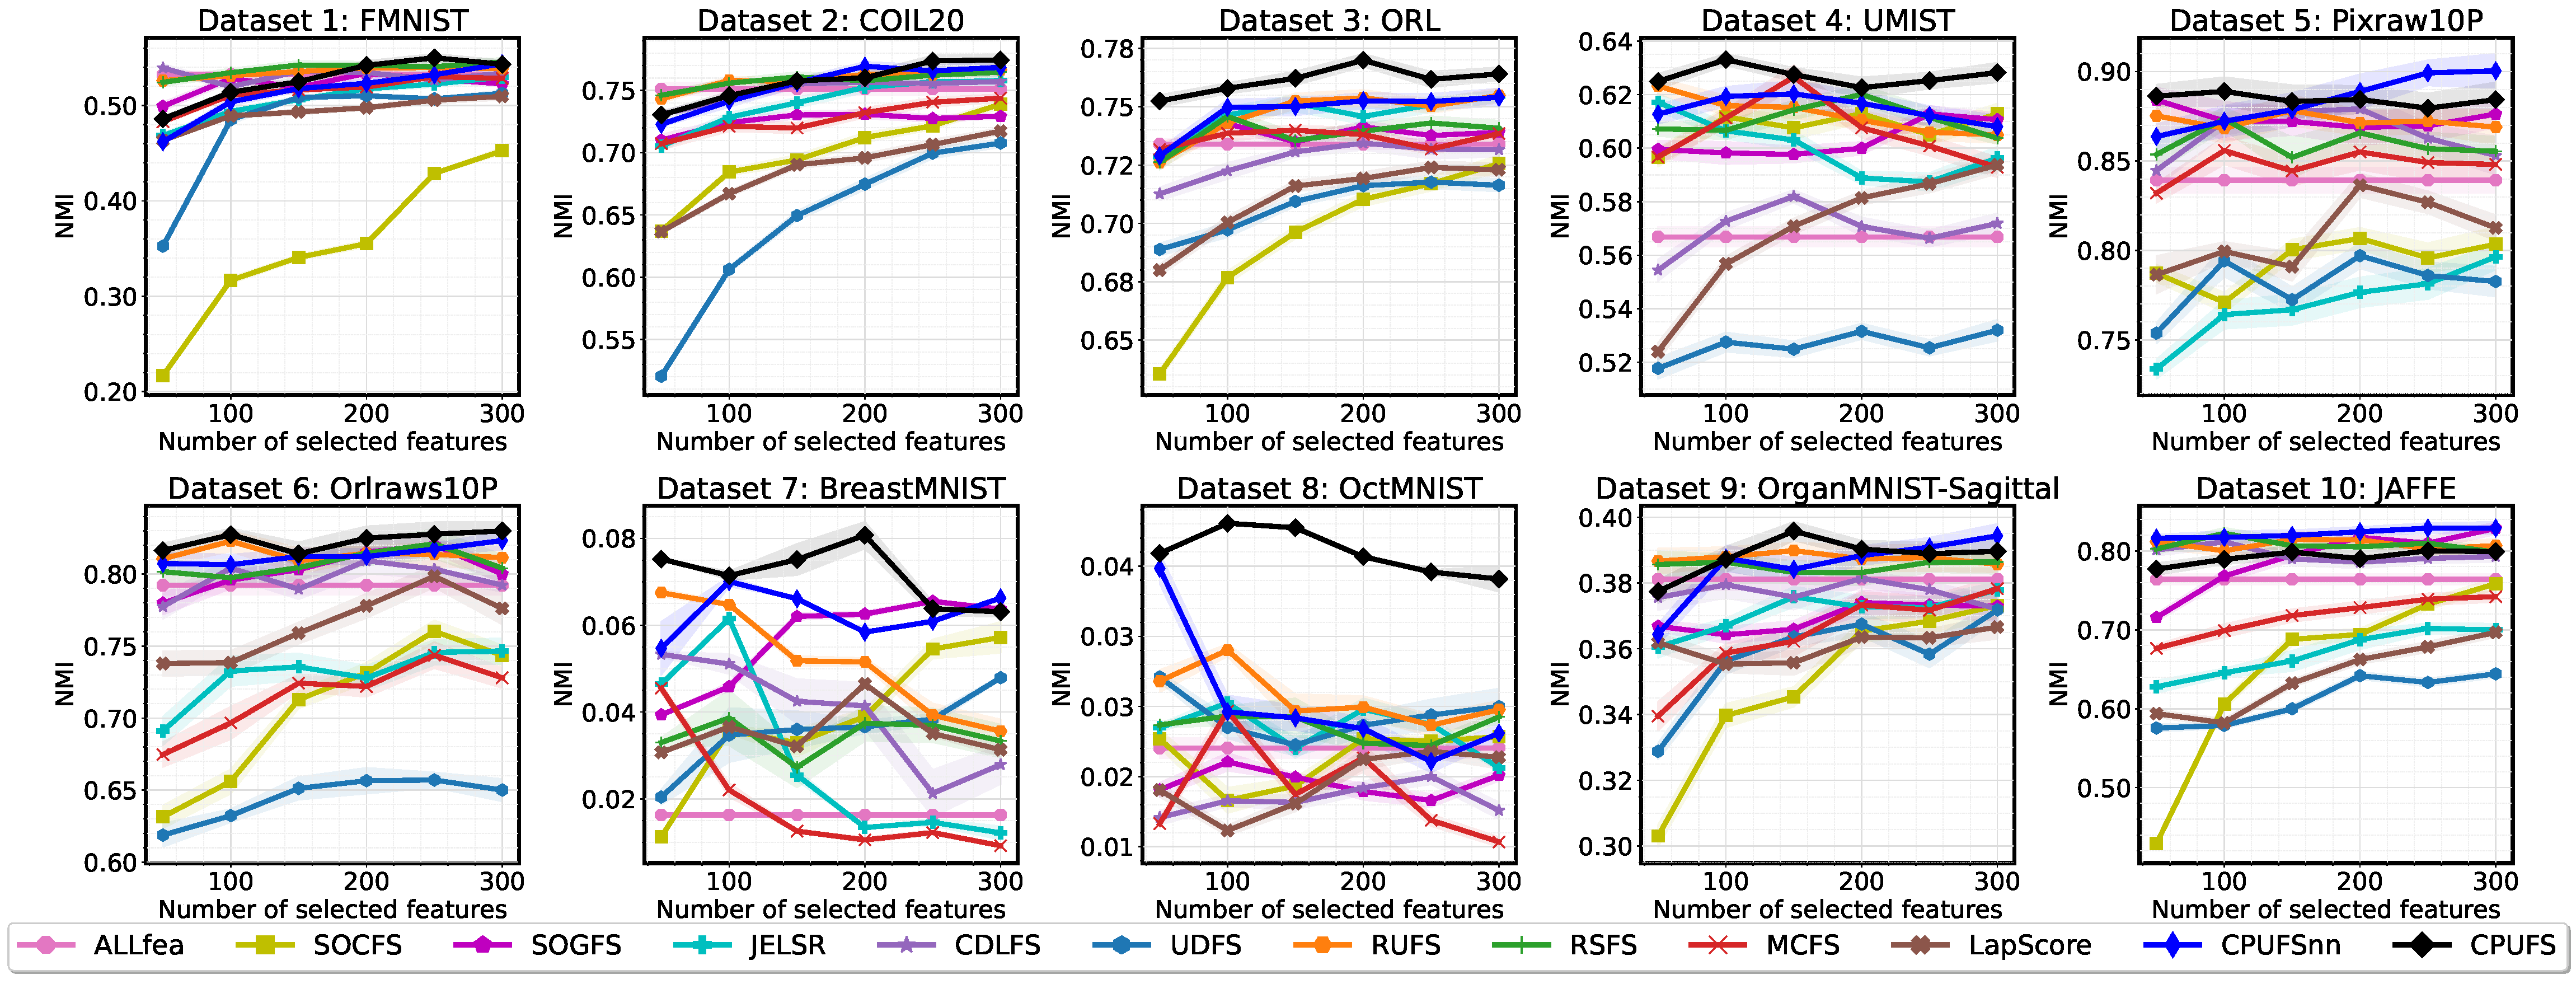
\includegraphics[width=\linewidth]{figures/CPUFS/NMIACC/PAMI_NMI.pdf}
    \caption{NMI}
    \label{fig:cpufs-nmi}
\end{sidewaysfigure}

\begin{sidewaysfigure}
    \centering
    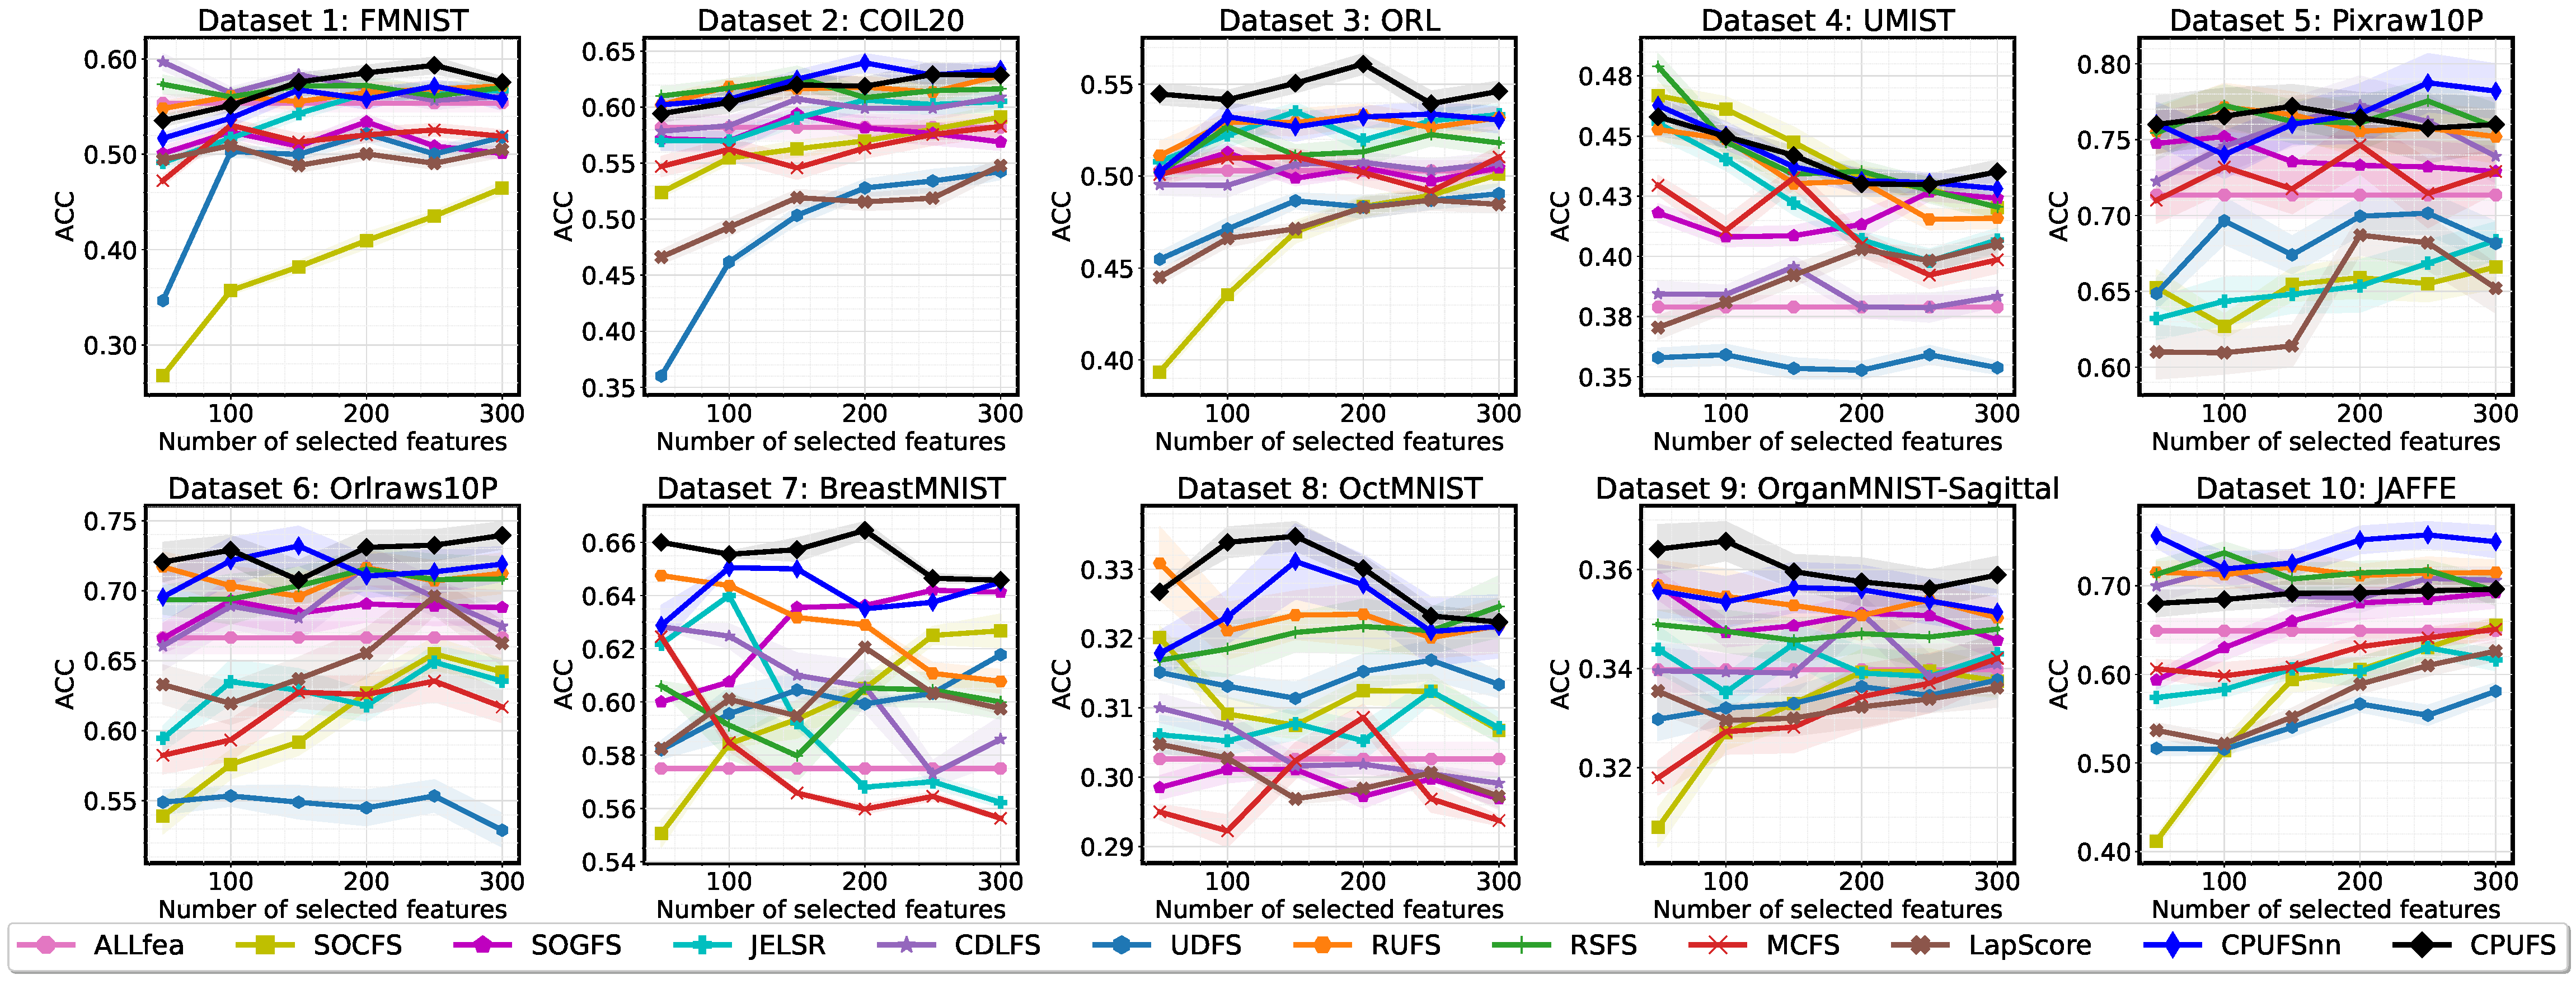
\includegraphics[width=\linewidth]{figures/CPUFS/NMIACC/PAMI_ACC.pdf}
    \caption{ACC}
    \label{fig:cpufs-acc}
\end{sidewaysfigure}

\subsection{实验二:参数敏感度分析}
\esubsection{Experiment 2: Parameter Sensitivity Analysis}
在这一小节,我们分析CPUFS模型中的参数$\nu$,$\alpha$以及$\beta$对特征选择性能的影响。具体来说,我们交替地在范围$\{10^{-2},10^{-1},1,10,10^{2}\}$内调整这些参数的其中之一,并固定其余所有参数为$1$,然后我们记录所有可能的参数组合下CPUFS的特征选择性能(由NMI来体现)。由于相似的实验结果可以在不同数据集上观测到,为了节省空间,我们只报告在FashionMNIST和UMIST数据集上的实验结果。实验结果如\reffig{fig:sensitivity}所示。由\reffig{fig:sensitivity},我们可以得出以下结论。
\begin{enumerate*}
\item 在FashionMNIST数据集上,当所选特征的数量较低时(比方说$50$或$100$),CPUFS的性能对这些参数相对敏感,而在其它情况下CPUFS的性能对这些参数并不敏感。此外,CPUFS的性能与所选特征的数量大致呈显正相关关系。
\item 在UMIST数据集上,CPUFS的性能对这些参数均相对不敏感,并且相对于所选功能的数量也不存在显著的相关性。
\end{enumerate*}

\begin{figure}[!ht]
\centering
% \subfloat[null]{
\includegraphics[width=0.33\linewidth]{figures/CPUFS/visualization/feaOriginal_ORL.pdf}}
% \subfloat[null]{
\includegraphics[width=0.33\linewidth]{figures/CPUFS/visualization/feaOriginal_ORL.pdf}}
% \subfloat[null]{
\includegraphics[width=0.33\linewidth]{figures/CPUFS/visualization/feaOriginal_ORL.pdf}}\\
% \subfloat[null]{
\includegraphics[width=0.33\linewidth]{figures/CPUFS/visualization/feaOriginal_ORL.pdf}}
% \subfloat[null]{
\includegraphics[width=0.33\linewidth]{figures/CPUFS/visualization/feaOriginal_ORL.pdf}}
% \subfloat[null]{
\includegraphics[width=0.33\linewidth]{figures/CPUFS/visualization/feaOriginal_ORL.pdf}}
\subfloat[FashionMNIST ($\nu$)\label{fig:f1}] {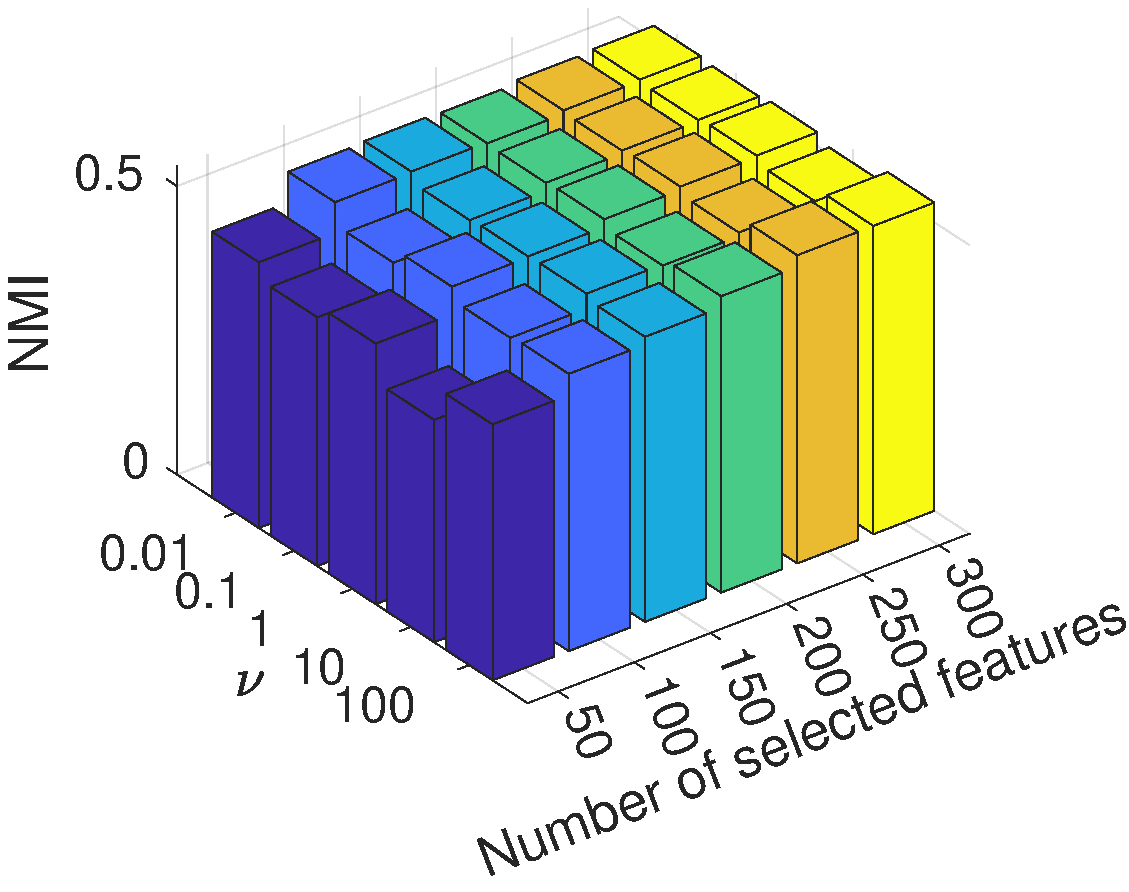
\includegraphics[width=0.33\linewidth]{figures/CPUFS/sensitivity/fmnist_nu.pdf}}
\subfloat[FashionMNIST ($\alpha$)\label{fig:f2}]{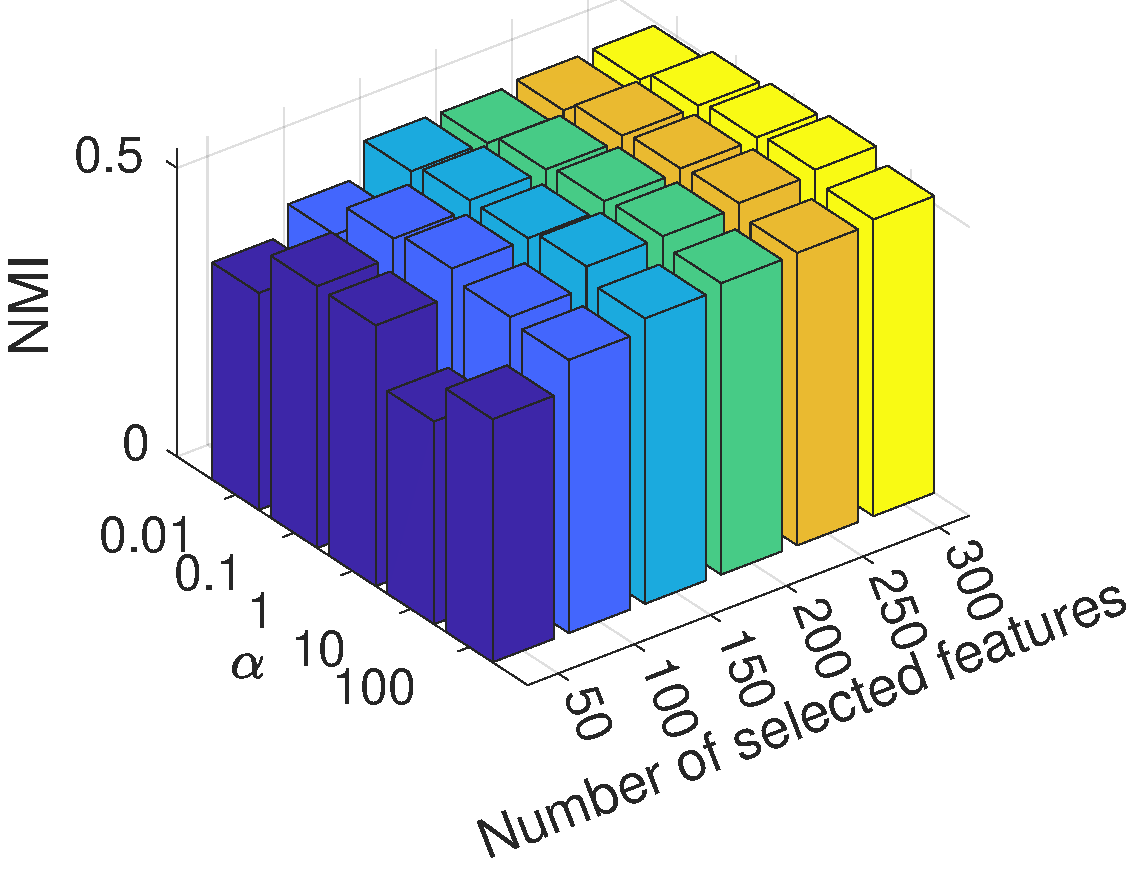
\includegraphics[width=0.33\linewidth]{figures/CPUFS/sensitivity/fmnist_alpha.pdf}}
\subfloat[FashionMNIST ($\beta$)\label{fig:f3}]{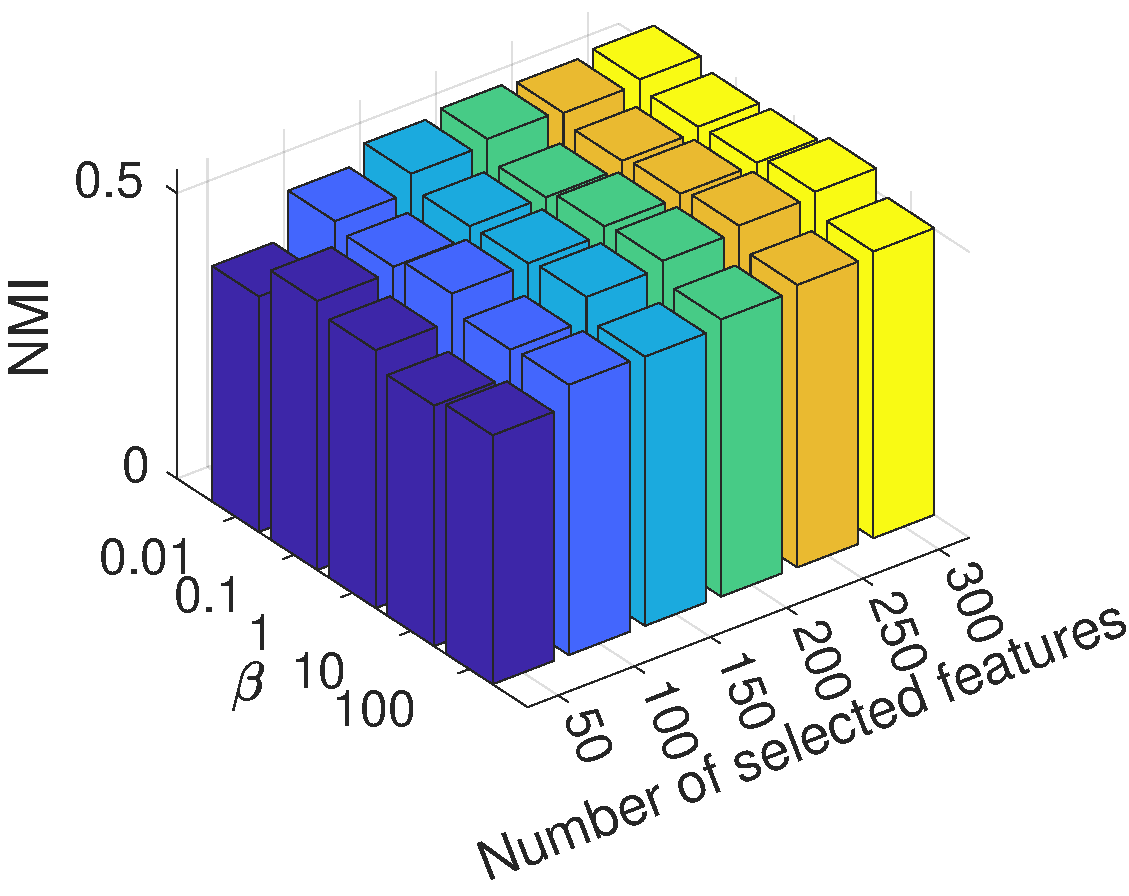
\includegraphics[width=0.33\linewidth]{figures/CPUFS/sensitivity/fmnist_beta.pdf}}\\
\subfloat[UMIST ($\nu$)\label{fig:w1}] {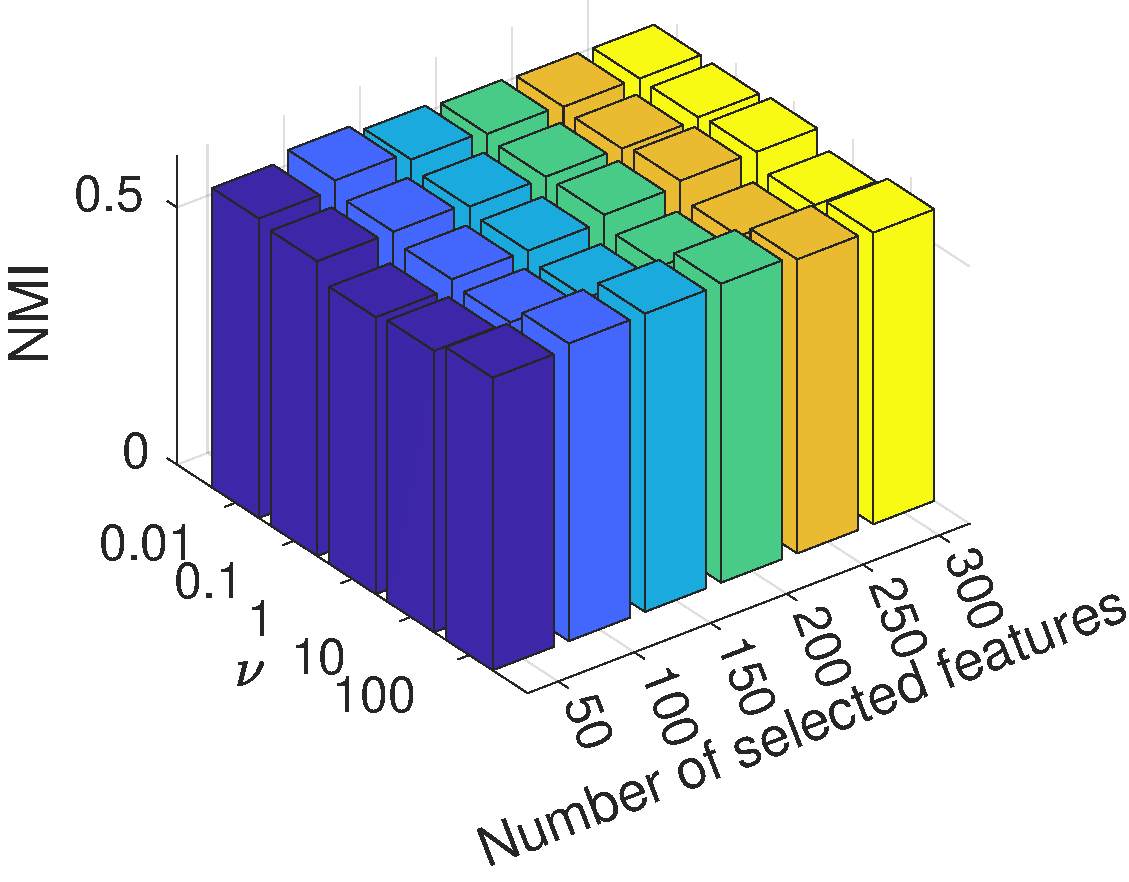
\includegraphics[width=0.33\linewidth]{figures/CPUFS/sensitivity/umist_nu.pdf}}
\subfloat[UMIST ($\alpha$)\label{fig:w2}]{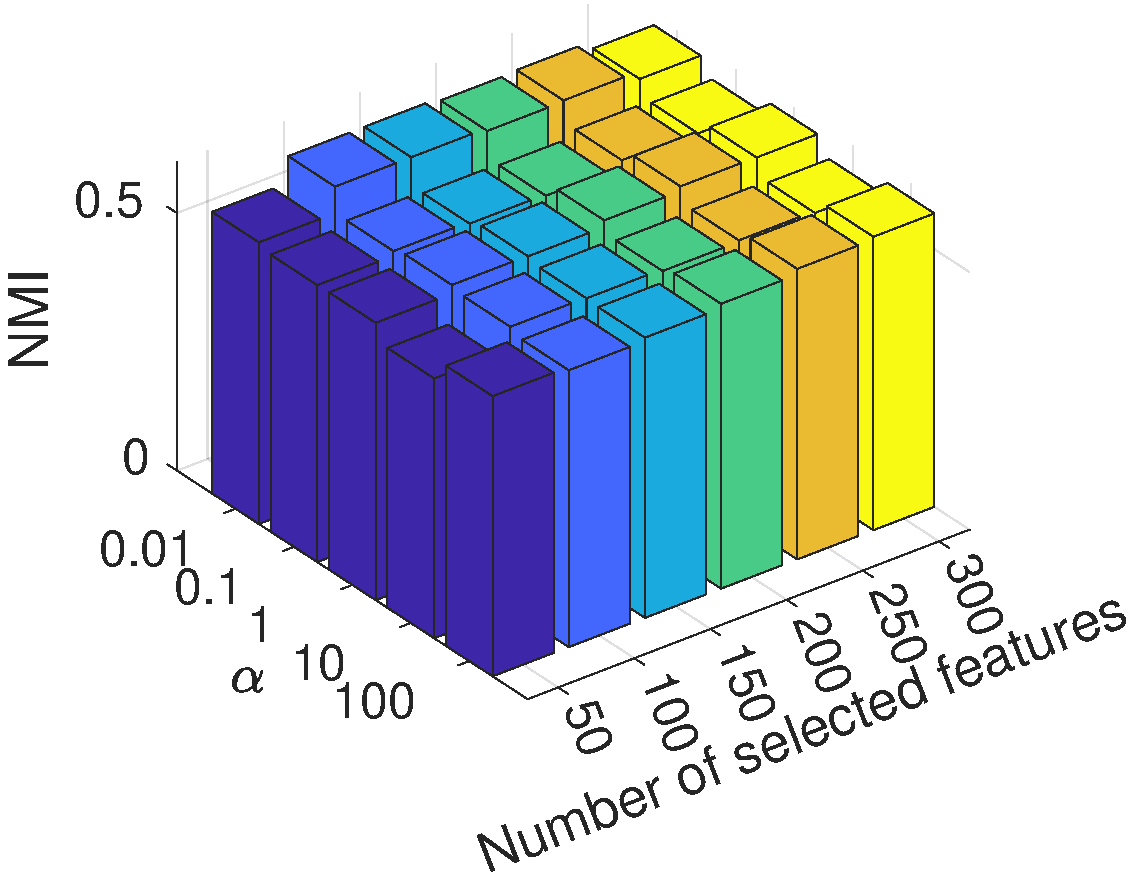
\includegraphics[width=0.33\linewidth]{figures/CPUFS/sensitivity/umist_alpha.pdf}}
\subfloat[UMIST ($\beta$)\label{fig:w3}]{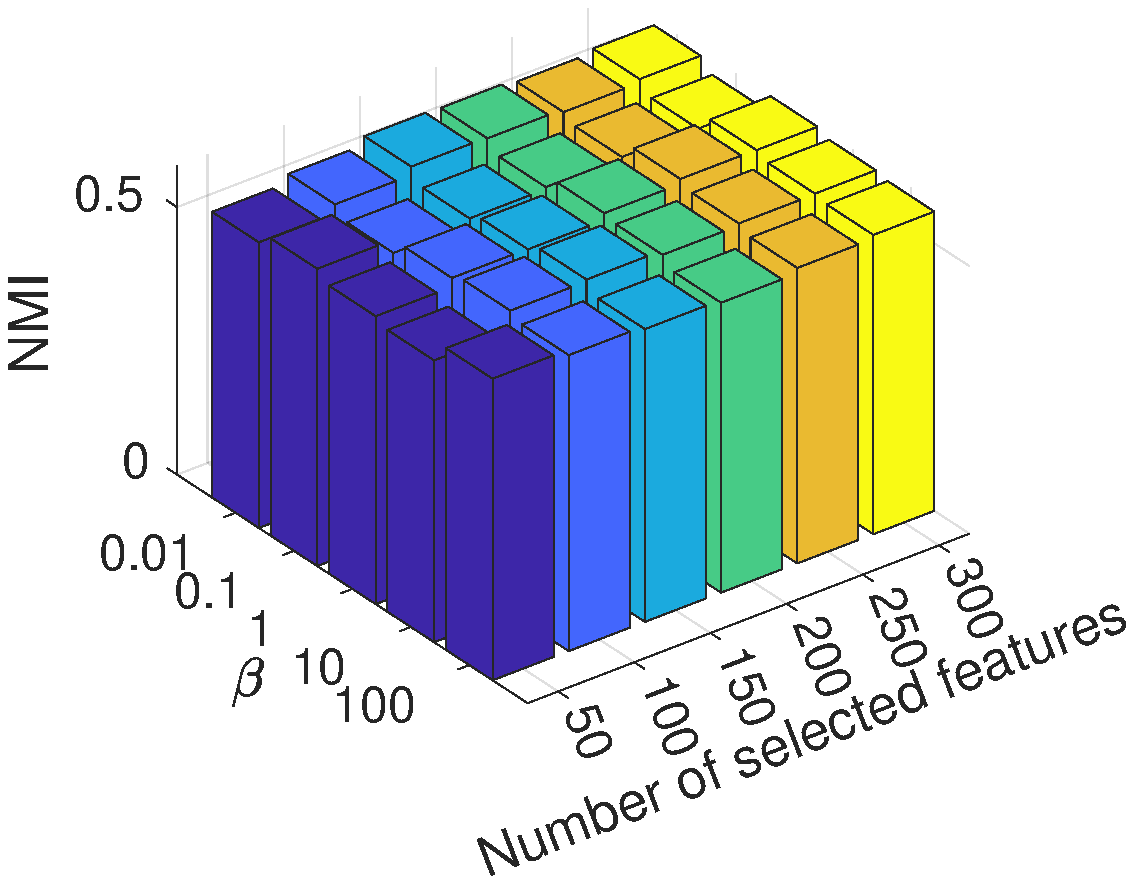
\includegraphics[width=0.33\linewidth]{figures/CPUFS/sensitivity/umist_beta.pdf}}\\
\subfloat[COIL20 ($\nu$)\label{fig:l1}] {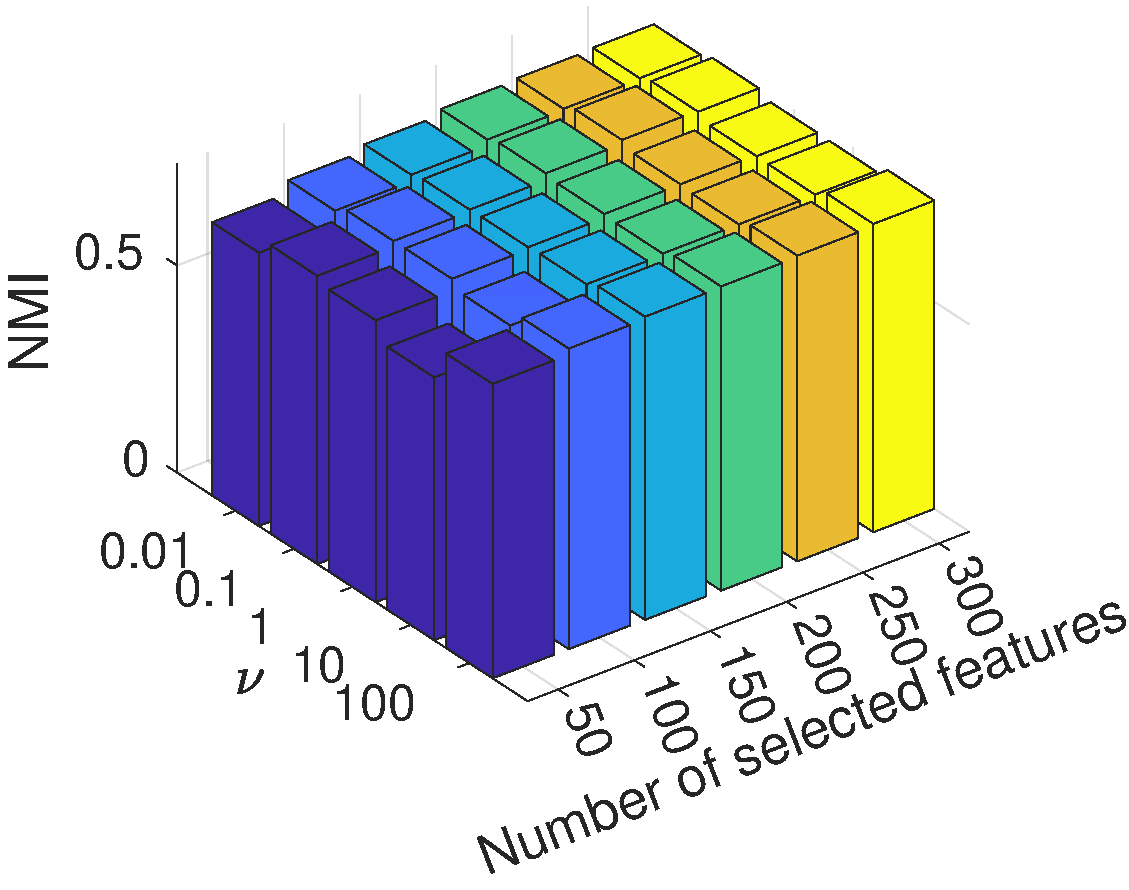
\includegraphics[width=0.33\linewidth]{figures/CPUFS/sensitivity/COIL20_nu.pdf}}
\subfloat[COIL20 ($\alpha$)\label{fig:l2}]{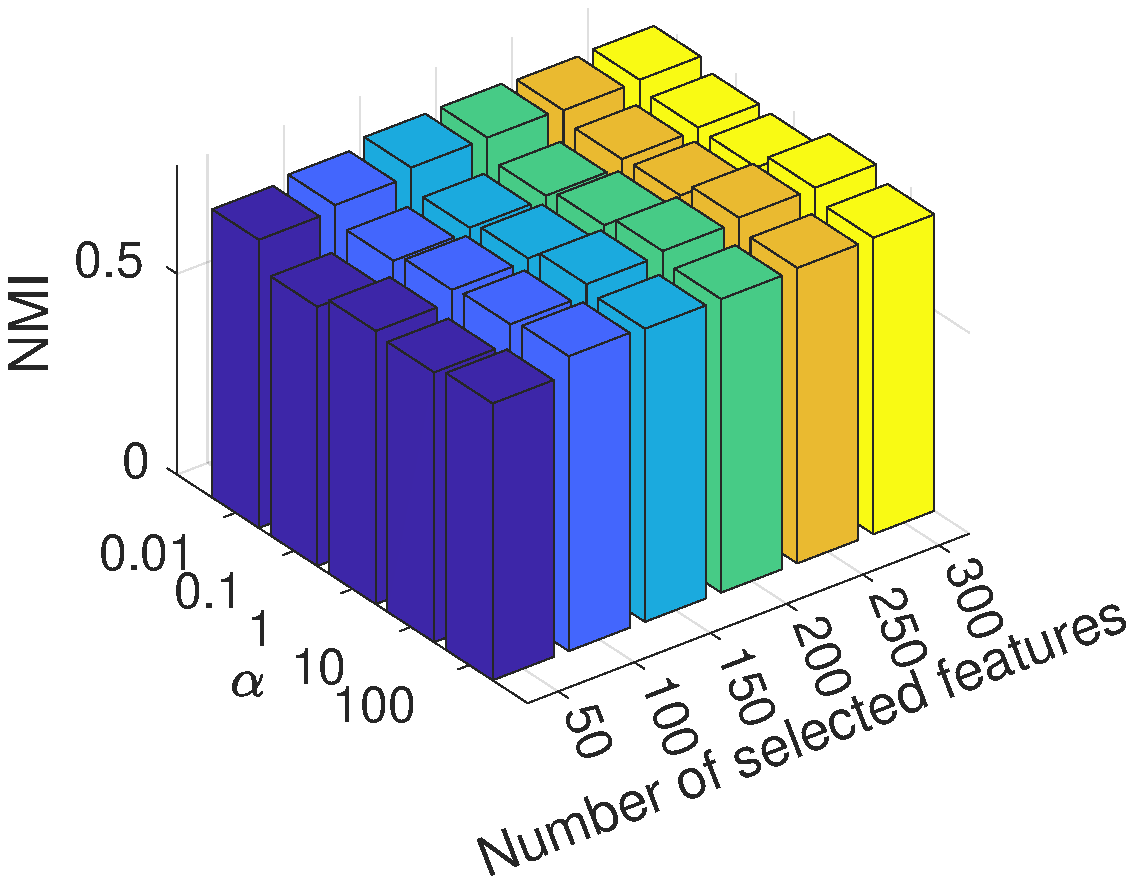
\includegraphics[width=0.33\linewidth]{figures/CPUFS/sensitivity/COIL20_alpha.pdf}}
\subfloat[COIL20 ($\beta$)\label{fig:l3}]{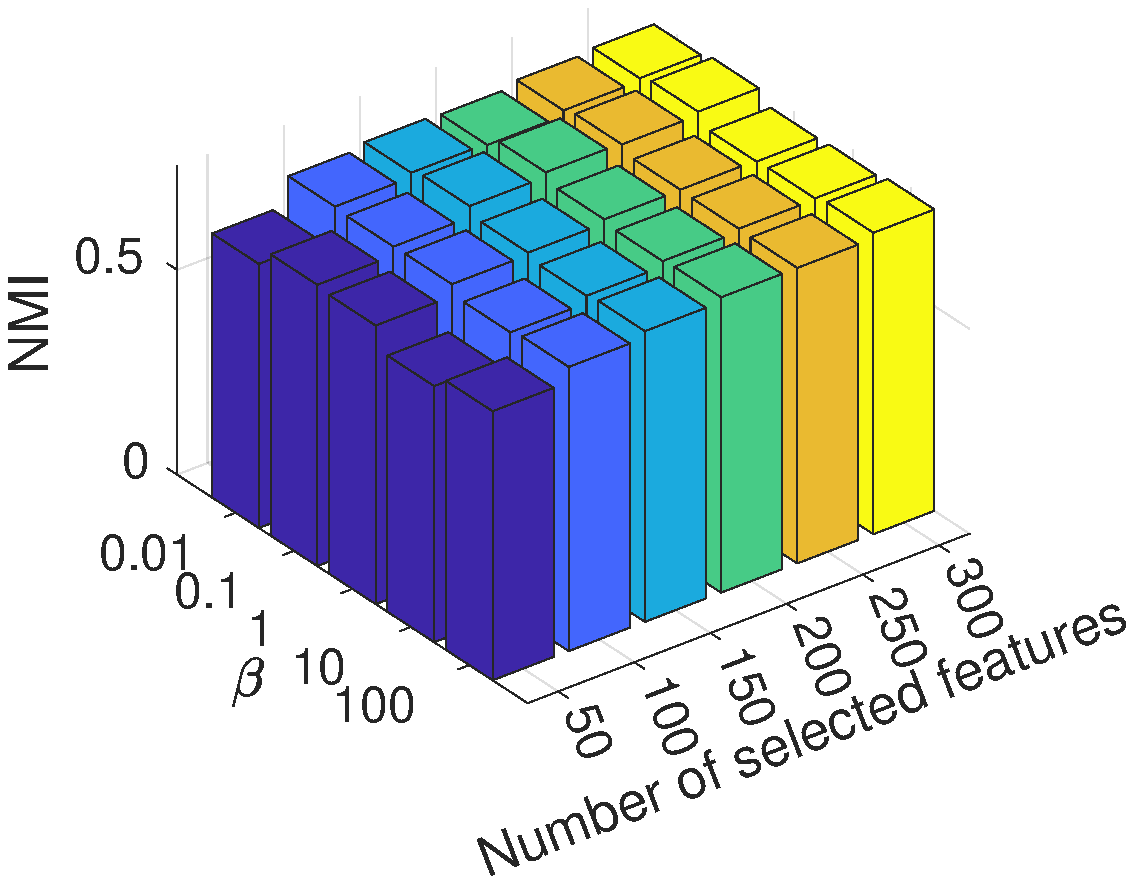
\includegraphics[width=0.33\linewidth]{figures/CPUFS/sensitivity/COIL20_beta.pdf}}
\caption{\mbox{CPUFS在FashionMNIST,UMIST和COIL20数据集上的参数敏感度分析}}
\label{fig:sensitivity}
\end{figure}

\subsection{实验三:运行时间分析}
\esubsection{Experiment 3: Running Time Analysis}
在本节中,我们分析所提出的CPUFS方法的运行时间。我们曾在\refsection{sec:companal}分析道,CPUFS的计算复杂性与数据中的特征数量中呈线性关系,而某些已有的方法可能呈三次关系。为了验证我们的分析,我们在Pixraw10P和Orlraws10P数据集上运行CPUFS,NDFS,UDFS和RSFS(这些数据集在所有数据集中具有最大的特征数量,因此它们更适合于比较运行时间)。具体来讲,我们将所有方法的所有可调参数固定为$1$,然后我们记录这四个方法在这两个数据集上的$50$步迭代内的运行时间。实验结果如\reffig{fig:runtime}(a)和\reffig{fig:runtime}(b)所示。我们观察到,我们提出的CPUFS方法与NDFS,UDFS和RSFS相比,需要明显更少的优化时间,而这清楚地验证了我们的理论复杂性分析。

\subsection{实验四:收敛性分析}
\esubsection{Experiment 4: Convergence Analysis}
在本节中,我们经验地研究\refalg{alg:cpufs}的收敛速度。具体来讲,我们在FashionMNIST数据集上运行CPUFS,并将其所有参数固定为$1$,然后记录其目标函数值在$105$步迭代内的变化趋势。相应的收敛曲线如\reffig{fig:runtime}(c)所示。从图中我们可以发现,目标函数值是单调减少的。更具体来讲,目标函数值在开始时迅速下降,然后稳定地降低到一个平稳点。这验证了我们推导的收敛理论\reftheorem{thm:conv}。此外,我们还可以从\reffig{fig:runtime}(c)中发现目标函数值在仅数十次迭代中的便降至较低水平。这确保了整个特征选择过程的效率。

\begin{figure}[!ht]
\centering
\subfloat[Pixraw10P\label{fig:r1}]{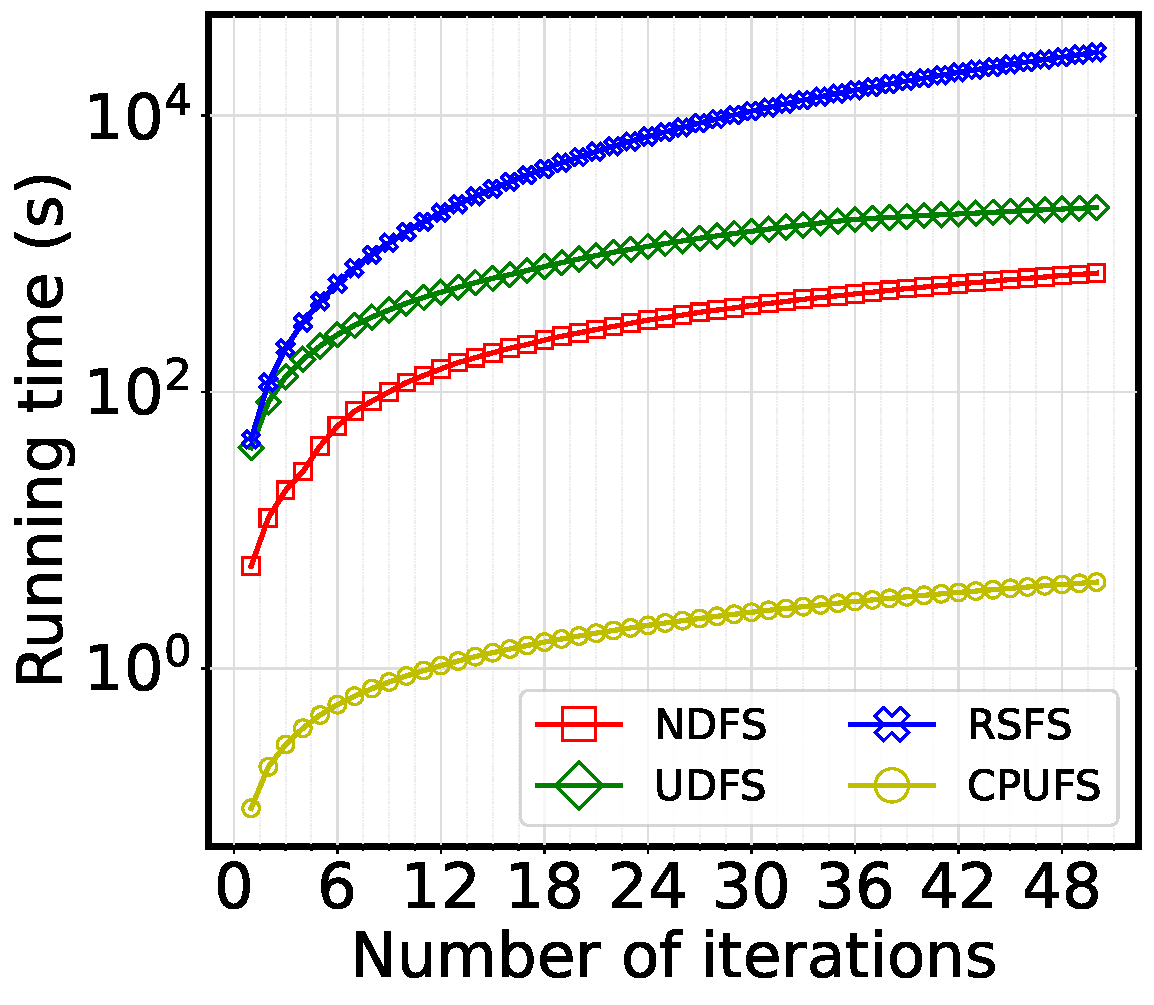
\includegraphics[width=0.33\linewidth]{figures/CPUFS/runtime/CPUFStime_Pixraw10P.pdf}}
\subfloat[Orlraws10P\label{fig:r2}]{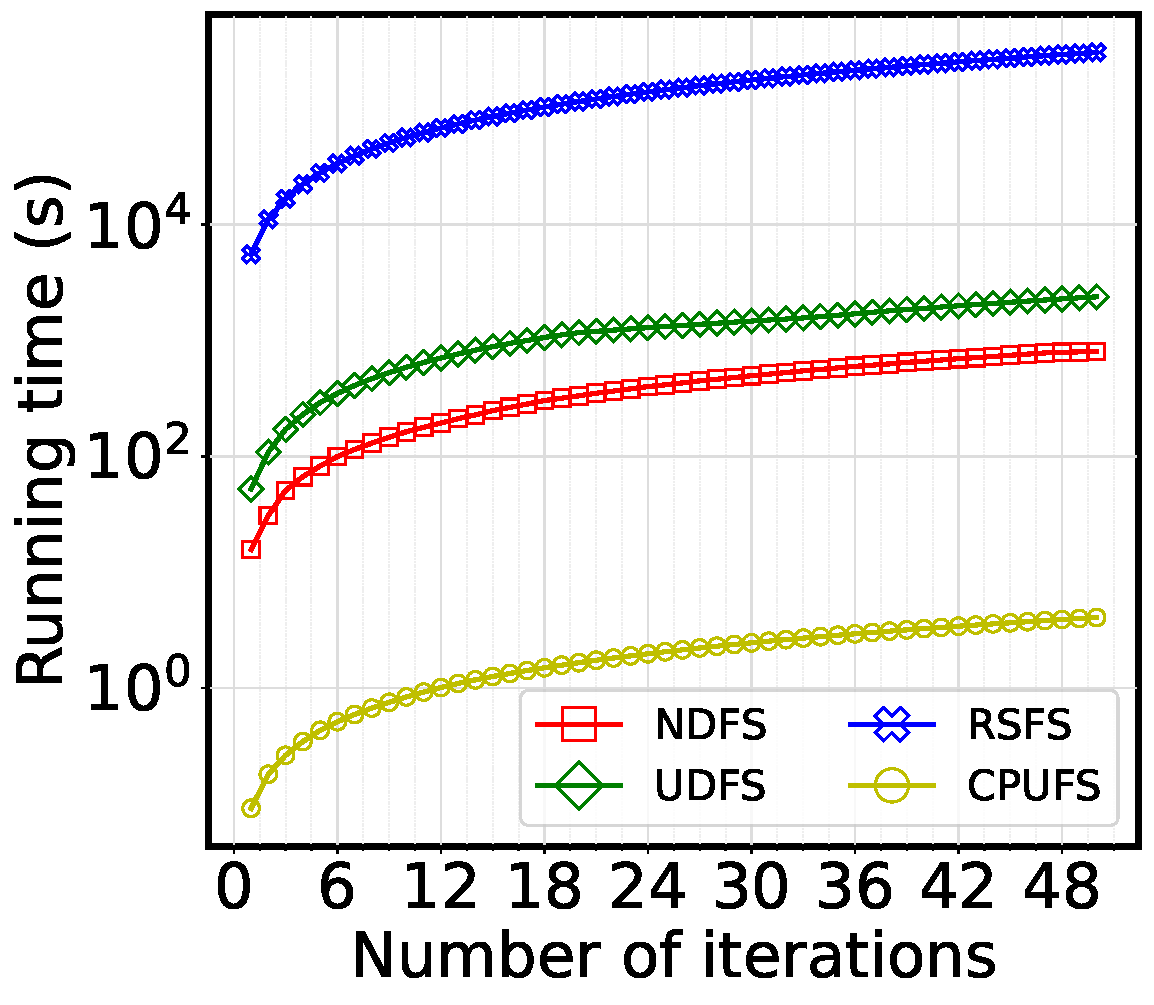
\includegraphics[width=0.33\linewidth]{figures/CPUFS/runtime/CPUFStime_Orlraws10P.pdf}}
\subfloat[JAFFE\label{fig:r3}]{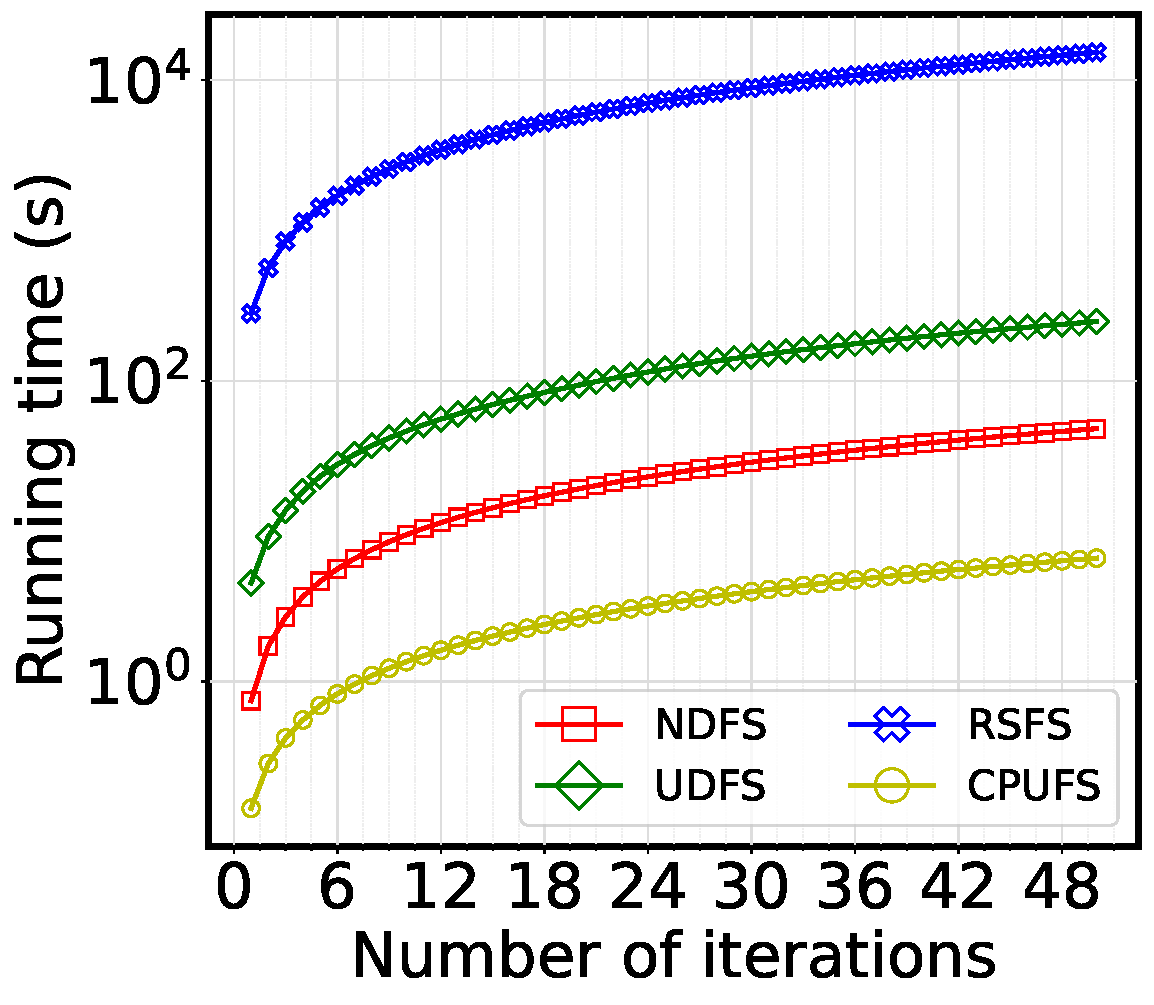
\includegraphics[width=0.33\linewidth]{figures/CPUFS/runtime/CPUFStime_Jaffe.pdf}}
\caption{CPUFS在Pixraw10P,Orlraws10P和JAFFE数据集上的运行时间分析}
\label{fig:runtime}
\end{figure}

\begin{figure}[!ht]
    \centering
    \subfloat[FashionMNIST\label{fig:c1}]{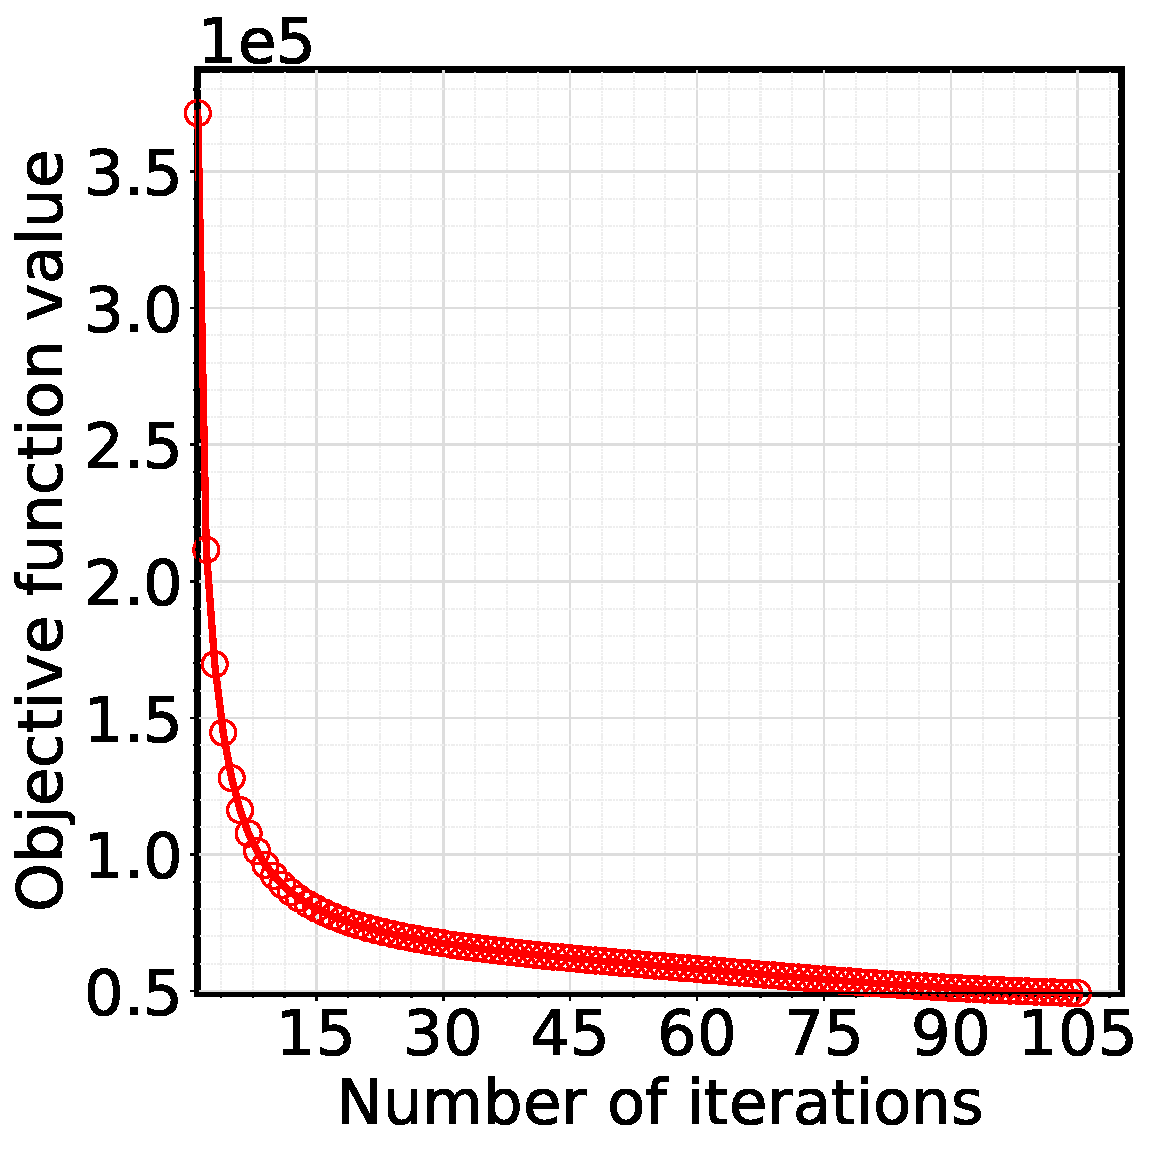
\includegraphics[width=0.33\linewidth]{figures/CPUFS/convergence/loss_fmnist.pdf}}
    \subfloat[UMIST\label{fig:c2}]{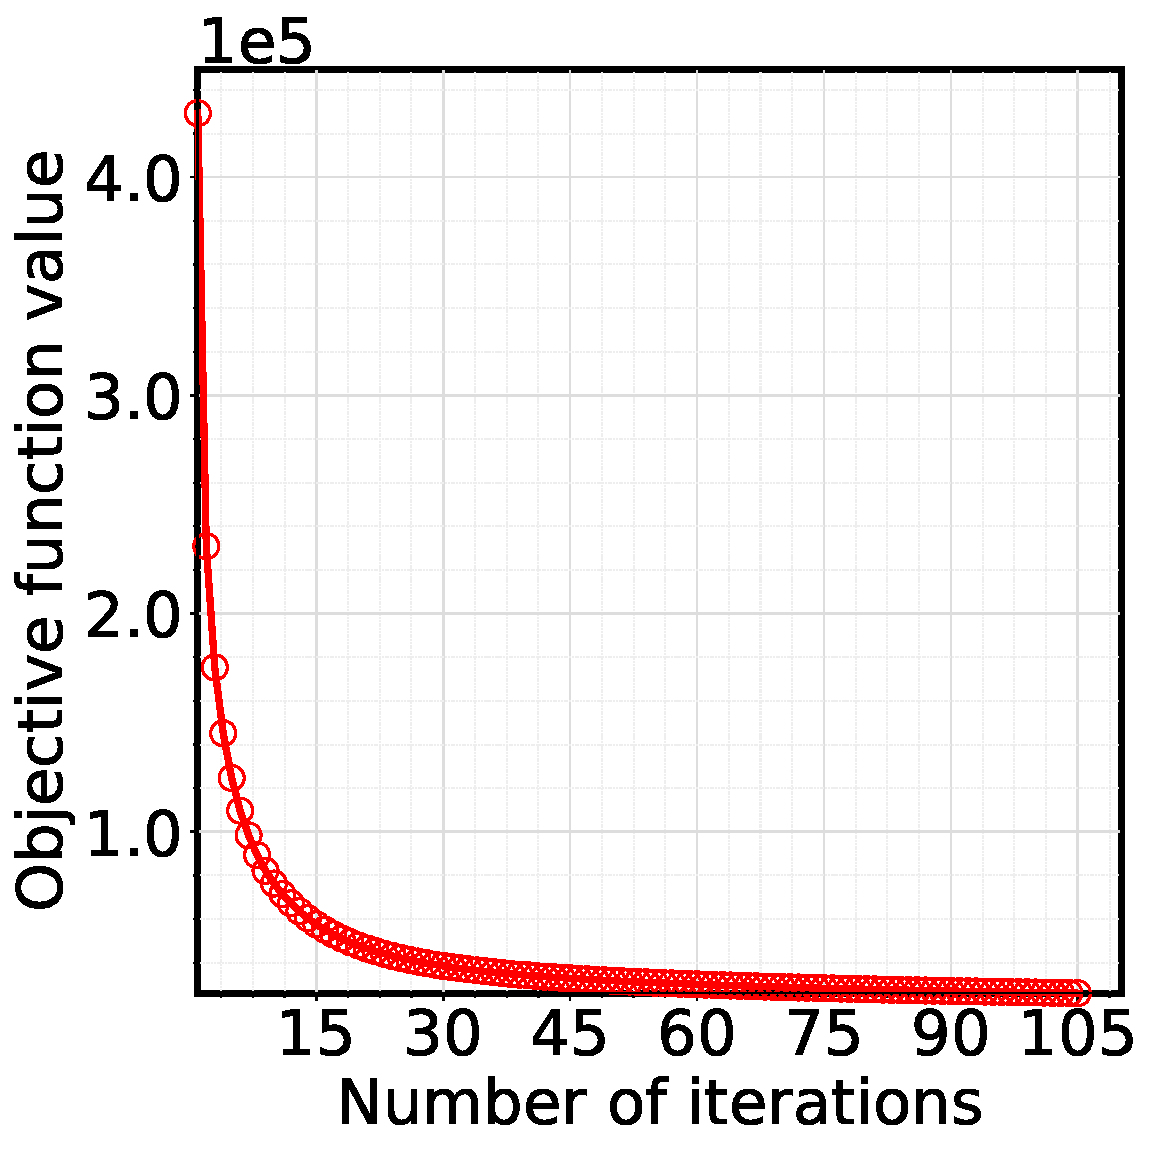
\includegraphics[width=0.33\linewidth]{figures/CPUFS/convergence/loss_umist.pdf}}
    \subfloat[COIL20\label{fig:c3}]{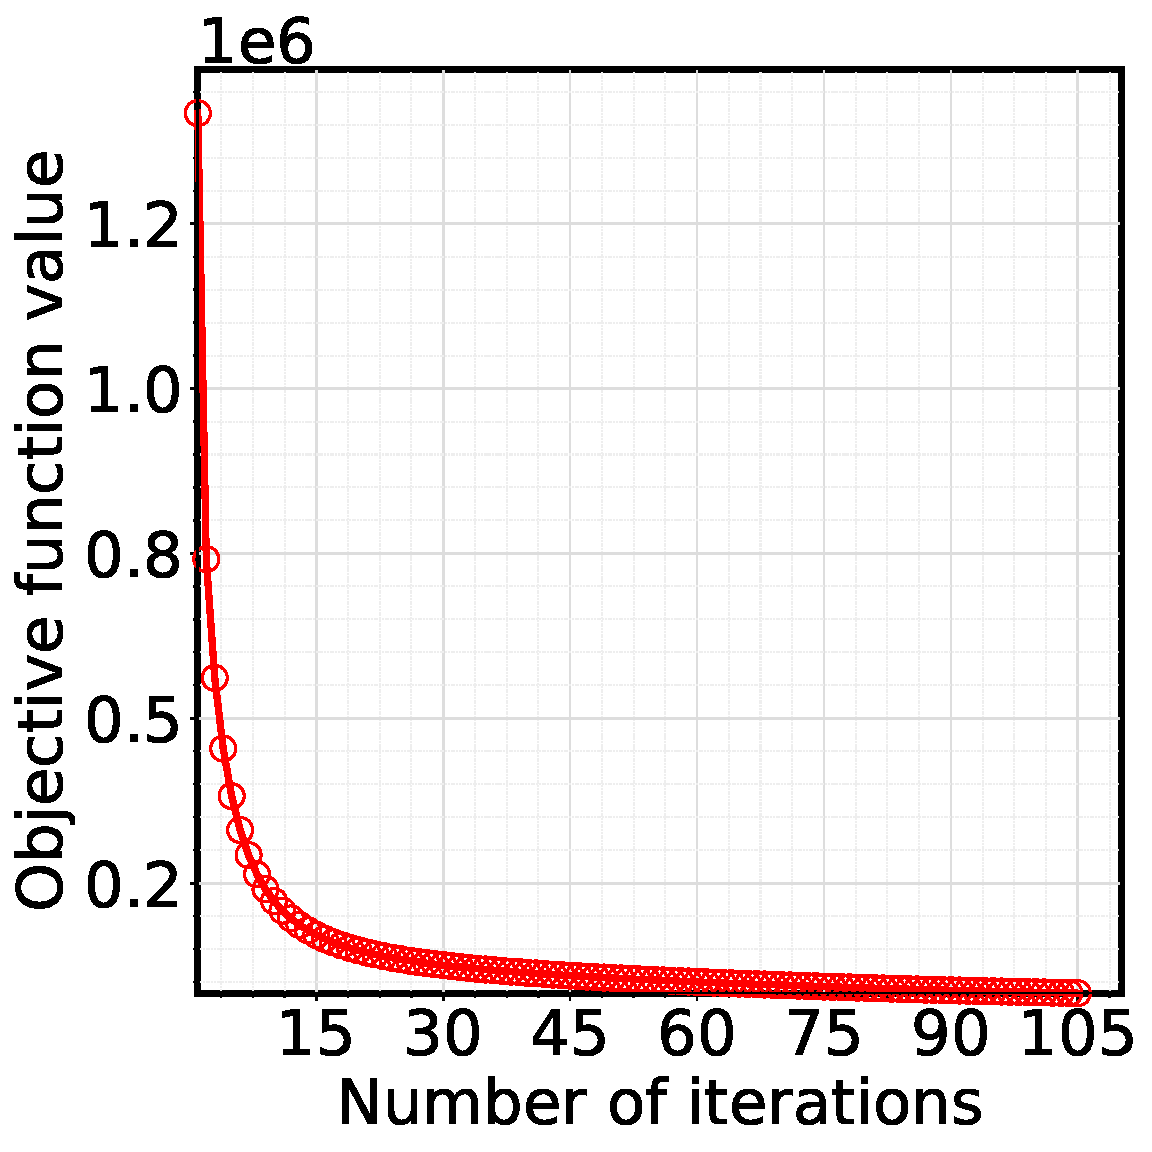
\includegraphics[width=0.33\linewidth]{figures/CPUFS/convergence/loss_COIL20.pdf}}
    \caption{CPUFS在FashionMNIST,UMIST和COIL20数据集上的收敛性分析}
    \label{fig:converge}
\end{figure}

\subsection{实验五:被选择特征的可视化}
\esubsection{Experiment 5: Selected Feature Visualization}
我们曾在\refsection{sec:design2}理论地分析道,在CPUFS模型中,来自原始二维数据的同一行或同一列的特征的特征重要性权重是相互关联的。我们现在实验地展示了这种相关性在实际情况下的表现如何。具体来讲,对于某一数据集,我们首先检索$300$个就NMI而言表现最好的特征(也就是说,这$300$个特征刚好就是达到\reffig{fig:clusnmi}中性能的那些),然后我们从该数据集随机采样一张图像并掩盖这张图像上的这$300$个特征。由于我们的方法与RUFS相对较为相似,因此我们还使用了同样的方法可视化了RUFS选择的特征。为了充分说明我们方法的特别之处,我们在ORL,JAFFE,OCTMNIST,FashionMNIST,COIL20,BreastMNIST,Pixraw10P以及Orlraws10P这八个数据集上进行了上述实验。实验结果如\reftab{tab:visulization}所示。可以看出,由我们的CPUFS方法所选择的特征在空间上具有较强的相关性:
\begin{enumerate*}
    \item 在ORL数据集上,被选择的特征更倾向于聚集在一个较小的矩形子区域内;
    \item 在JAFFE和Orlraws10P数据集上,被选择的特征显示出了明显的网格状结构;
    \item 在OCTMNIST和BreastMNIST数据集上,被选择的特征更倾向于聚集在一起;
    \item 在FashionMNIST,COIL20以及Pixraw10P数据集上,被选择的特征在垂直方向上具有清晰的结构特性。
\end{enumerate*}
然而,由RUFS选择出来的特征却没有显示出这样的效果。这种现象充分展示了基于张量的无监督特征选择方法的有效性。我们认为,CPUFS的性能提升主要归功于其所选特征的更好结构。

\begin{figure}[!ht]
    \centering
    \subfloat[ORL] {
\includegraphics[width=0.32\linewidth]{figures/CPUFS/visualization/feaOriginal_ORL.pdf}}
    \hspace{0.01\linewidth}
    \subfloat[ORL (CPUFS)]{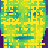
\includegraphics[width=0.32\linewidth]{figures/CPUFS/visualization/feaCPUFS_ORL.pdf}}
    \hspace{0.01\linewidth}
    \subfloat[ORL (RUFS)] {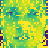
\includegraphics[width=0.32\linewidth]{figures/CPUFS/visualization/feaRUFS_ORL.pdf}}\\
    \subfloat[JAFFE] {\includegraphics[width=0.32\linewidth]{figures/CPUFS/visualization/feaOriginal_jaffe.pdf}}
    \hspace{0.01\linewidth}
    \subfloat[JAFFE (CPUFS)]{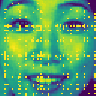
\includegraphics[width=0.32\linewidth]{figures/CPUFS/visualization/feaCPUFS_JAFFE.pdf}}
    \hspace{0.01\linewidth}
    \subfloat[JAFFE (RUFS)] {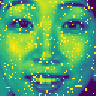
\includegraphics[width=0.32\linewidth]{figures/CPUFS/visualization/feaRUFS_JAFFE.pdf}}\\
    \subfloat[OCTMNIST] {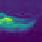
\includegraphics[width=0.32\linewidth]{figures/CPUFS/visualization/feaOriginal_octmnist.pdf}}
    \hspace{0.01\linewidth}
    \subfloat[OCTMNIST (CPUFS)]{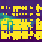
\includegraphics[width=0.32\linewidth]{figures/CPUFS/visualization/feaCPUFS_octmnist.pdf}}
    \hspace{0.01\linewidth}
    \subfloat[OCTMNIST (RUFS)] {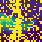
\includegraphics[width=0.32\linewidth]{figures/CPUFS/visualization/feaRUFS_octmnist.pdf}}\\
    \subfloat[FashionMNIST] {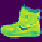
\includegraphics[width=0.32\linewidth]{figures/CPUFS/visualization/feaOriginal_fmnist.pdf}}
    \hspace{0.01\linewidth}
    \subfloat[FashionMNIST (CPUFS)]{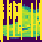
\includegraphics[width=0.32\linewidth]{figures/CPUFS/visualization/feaCPUFS_fmnist.pdf}}
    \hspace{0.01\linewidth}
    \subfloat[FashionMNIST (RUFS)] {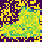
\includegraphics[width=0.32\linewidth]{figures/CPUFS/visualization/feaRUFS_fmnist.pdf}}\\
\end{figure}
\begin{figure}[!ht]
    \ContinuedFloat
    \centering
    \subfloat[COIL20] {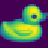
\includegraphics[width=0.32\linewidth]{figures/CPUFS/visualization/feaOriginal_COIL20.pdf}}
    \hspace{0.01\linewidth}
    \subfloat[COIL20 (CPUFS)]{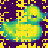
\includegraphics[width=0.32\linewidth]{figures/CPUFS/visualization/feaCPUFS_COIL20.pdf}}
    \hspace{0.01\linewidth}
    \subfloat[COIL20 (RUFS)] {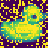
\includegraphics[width=0.32\linewidth]{figures/CPUFS/visualization/feaRUFS_COIL20.pdf}}\\
    \subfloat[BreastMNIST] {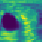
\includegraphics[width=0.32\linewidth]{figures/CPUFS/visualization/feaOriginal_breastmnist.pdf}}
    \hspace{0.01\linewidth}
    \subfloat[BreastMNIST (CPUFS)]{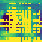
\includegraphics[width=0.32\linewidth]{figures/CPUFS/visualization/feaCPUFS_breastmnist.pdf}}
    \hspace{0.01\linewidth}
    \subfloat[BreastMNIST (RUFS)] {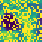
\includegraphics[width=0.32\linewidth]{figures/CPUFS/visualization/feaRUFS_breastmnist.pdf}}\\
    \subfloat[Pixraw10P] {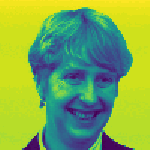
\includegraphics[width=0.32\linewidth]{figures/CPUFS/visualization/feaOriginal_pixraw10P.pdf}}
    \hspace{0.01\linewidth}
    \subfloat[Pixraw10P (CPUFS)]{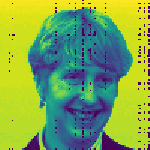
\includegraphics[width=0.32\linewidth]{figures/CPUFS/visualization/feaCPUFS_pixraw10P.pdf}}
    \hspace{0.01\linewidth}
    \subfloat[Pixraw10P (RUFS)] {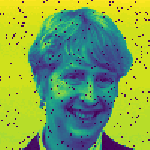
\includegraphics[width=0.32\linewidth]{figures/CPUFS/visualization/feaRUFS_pixraw10P.pdf}}\\
    \subfloat[Orlraws10P] {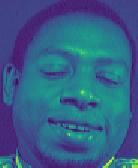
\includegraphics[width=0.32\linewidth]{figures/CPUFS/visualization/feaOriginal_orlraws10P.pdf}}
    \hspace{0.01\linewidth}
    \subfloat[Orlraws10P (CPUFS)]{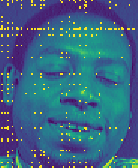
\includegraphics[width=0.32\linewidth]{figures/CPUFS/visualization/feaCPUFS_orlraws10P.pdf}}
    \hspace{0.01\linewidth}
    \subfloat[Orlraws10P (RUFS)] {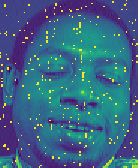
\includegraphics[width=0.32\linewidth]{figures/CPUFS/visualization/feaRUFS_orlraws10P.pdf}}\\
    \caption{CPUFS与RUFS所选择特征的可视化}
    \label{fig:visulization}
\end{figure}
\clearpage
\section{实验第二部分:无监督特征提取}
\esection{Experiment Part II: Unsupervised Feature Extraction}
\subsection{实验一:与\texorpdfstring{$\ell_{1}$}{L1}模型以及\texorpdfstring{$\ell_{2}$}{L2}模型的性能对比}
\esubsection{Experiment 1: Comparisons with \texorpdfstring{$\ell_{1}$}{L1} and \texorpdfstring{$\ell_{2}$}{L2} Models}
在这一小节,我们通过在不同的噪声情况下的图像分类和人脸识别任务来评估$\ell_{\infty}$相比于$\ell_{1}$与$\ell_{2}$模型的性能优劣。具体来讲,我们分别使用$\ell_{\infty}$,$\ell_{2}$以及$\ell_{1}$模型在\refsection{sec:noisy-data}中所提及的所有带噪声数据集中依据\refsection{sec:workflow}中介绍的工作流程进行特征提取。然后,我们基于被提取的特征使用$k$-NN分类器以及SVM分类器进行图像分类与人脸识别,并使用分类准确率来评估提取的特征的质量。为了缓解随机初始化所带来的随机效果,我们将每个模型运行三次,并报告平均结果。实验结果如\reftab{tab:coil},\reftab{tab:yale}以及\reftab{tab:umist}所示,其中粗体代表最佳的性能数值。从这些表格中,我们可以得出以下结论。

\begin{itemize}
    \item \textbf{我们提出的$\ell_{\infty}$模型非常有效。} 如表所示,在大多数情况下,我们提出的$\ell_{\infty}$模型相比于$\ell_{2}$以及$\ell_{1}$模型展现出了显著的性能提升。例如,在COIL(sp-10-20-30-40)数据集上,就$k$-NN ACC而言,$\ell_{\infty}$模型的性能相比于$\ell_{2}$以及$\ell_{1}$模型分别提升了$10\%$和$20\%$。除此之外,尽管$\ell_{\infty}$模型在YALE数据集的一些噪声情况下的性能不如$\ell_{1}$模型,但它的整体表现仍然很好,并且在很多情况下比$\ell_{2}$模型要好得多。这些现象充分说明了我们提出的$\ell_{\infty}$模型的有效性。
    \item \textbf{我们提出的$\ell_{\infty}$最适用于噪声情形。}我们可以发现,在三个没有施加噪声的数据集上,我们提出的$\ell_{\infty}$模型表现得并不是特别好。主要原因是由于我们提出的$\ell_{\infty}$模型致力于优化样本中具有最大拟合误差的那一个,而这似乎并不是在无噪声数据集下的明智选择。当数据中存在噪声时,我们的$\ell_{\infty}$模型会是一个较好的选择。
    \item \textbf{天下没有免费的午餐\ucite{wolpert1997no}。}正如我们所观察到的那样,尽管我们提出的$\ell_{\infty}$模型在COIL以及UMIST数据集上表现的相当出色,但它的性能在YALE数据集上并不如我们预期的那样优秀(尽管仍然可圈可点),而在该数据集上,$\ell_{1}$模型的表现较为突出。这表明不同的模型可能适用于不同类型的数据集。
\end{itemize}

\begin{table}[!ht]
        \caption{\mbox{与$\ell_{1}$以及$\ell_{2}$模型在COIL数据集上的性能对比}}
        \label{tab:coil}
        \centering
        \resizebox{\linewidth}{!}{%
            \begin{tabular}{lcccccc}
    \hline
    \multirow{2}{*}{Noise} & \multicolumn{3}{c}{$k$-NN ACC}                                                                         & \multicolumn{3}{c}{SVM ACC}                                                                            \\ \cline{2-7}
                           & $\ell_2$                         & $\ell_1$                         & $\ell_\infty$                    & $\ell_2$                         & $\ell_1$                         & $\ell_\infty$                    \\ \hline
    original               & \textbf{0.9208} & 0.8906                           & {0.8891}       & \textbf{0.9406} & 0.9065                           & 0.9198                           \\
    ms-5-10-20                  & 0.8560                           & 0.8560                           & \textbf{0.8810} & 0.9234                           & 0.9242                           & \textbf{0.9388} \\
    ms-10-10-10 & 0.8435 & 0.8240 & \textbf{0.8990} & 0.9234 & 0.8758 & \textbf{0.9500} \\
    ms-10-20-30 & 0.8224 & 0.7852 & \textbf{0.8406} & 0.9036 & 0.9133 & \textbf{0.9466} \\
    ms-10-30-50 & 0.8221 & 0.8013 & \textbf{0.8721} & 0.9031 & 0.9107 & \textbf{0.9339} \\
    ms-10-50-90 & 0.8128 & 0.7888 & \textbf{0.8664} & 0.9133 & 0.9008 & \textbf{0.9401} \\
    ms-20-20-20 & 0.8159 & 0.8073 & \textbf{0.8698} & 0.9112 & 0.9010 & \textbf{0.9378} \\
    ms-30-30-30 & 0.7901 & 0.8180 & \textbf{0.8768} & 0.9174 & 0.9104 & \textbf{0.9380} \\
    ms-40-40-40 & 0.8076 & 0.8193 & \textbf{0.8964} & 0.9190 & 0.9128 & \textbf{0.9570} \\
    ms-50-50-50 & 0.8250 & 0.8206 & \textbf{0.8680} & 0.9216 & 0.9216 & \textbf{0.9469} \\
    % ms010                  & 0.8068                           & \textbf{0.8836} & {0.8432}       & 0.7211                           & \textbf{0.9307} & 0.8076                           \\
    % ms020                  & 0.5659                           & \textbf{0.8766} & {0.8536}       & 0.4023                           & 0.6763                           & \textbf{0.7685} \\
    % sp002                  & 0.8453                           & 0.8305                           & \textbf{0.8664}       & \textbf{0.9276} & 0.9021                           & 0.9096                           \\
    % sp005                  & 0.8286                           & 0.8237                           & \textbf{0.8721} & 0.9021                           & 0.8938                           & \textbf{0.9026} \\
    % sp007                  & \textbf{0.8372} & 0.8172                           & {0.8076}       & 0.8661                           & 0.8792                           & \textbf{0.8932} \\
    % ms-0-0-0-90                 & 0.8576                           & 0.8375                           & \textbf{0.8826} & 0.9177                           & 0.8977                           & \textbf{0.9187} \\
    ms-5-10-15-20                 & 0.8285                           & 0.7830                           & \textbf{0.8969} & 0.9041                           & 0.8934                           & \textbf{0.9346} \\
    ms-10-10-10-10 & 0.8320 & 0.8391 & \textbf{0.8482} & \textbf{0.9260} & 0.9156 & 0.9115 \\
    ms-10-20-30-40                 & 0.7526                           & 0.7049                           & \textbf{0.8534} & 0.8945                           & 0.8734                           & \textbf{0.9352} \\
    % ms-10-20-30-90 & \textbf{0.7883} & 0.7513 & 0.7781 & 0.8971 & 0.8956 & \textbf{0.9216} \\
    % ms1239                 & \textbf{0.7883} & 0.7513                           & {0.7781}       & 0.8971                           & 0.8956                           & \textbf{0.9216} \\
    ms-10-30-50-70                 & 0.7940                           & 0.7776                           & \textbf{0.8555} & 0.8729                           & 0.9156                           & \textbf{0.9344} \\
    ms-20-20-20-20 & 0.7716 & \textbf{0.8247} & 0.8063 & 0.9078 & 0.9086 & \textbf{0.9245} \\
    ms-30-30-30-30 & 0.7615 & 0.7880 & \textbf{0.8010} & 0.9125 & 0.9159 & \textbf{0.9430} \\
    ms-40-40-40-40 & 0.7596 & 0.7802 & \textbf{0.8526} & 0.9201 & 0.9281 & \textbf{0.9549} \\
    ms-50-50-50-50 & 0.7721 & 0.7974 & \textbf{0.8104} & 0.9190 & 0.9143 & \textbf{0.9385} \\
    \hline\hline
    % sp-1-2-10                  & 0.8461                           & 0.8471                           & \textbf{0.8922} & 0.9180                           & 0.9005                           & \textbf{0.9292} \\
    sp-5-10-20 & 0.8029 & 0.8109 & \textbf{0.8839} & 0.9115 & 0.9026 & \textbf{0.9383} \\
    sp-10-10-10 & 0.7865 & 0.7492 & \textbf{0.8664} & 0.9065 & 0.8841 & \textbf{0.9320} \\
    sp-10-20-30 & 0.7969 & 0.7414 & \textbf{0.8766} & 0.8922 & 0.7859 & \textbf{0.9336} \\
    sp-10-30-50 & 0.7865 & 0.8318 & \textbf{0.8846} & 0.8992 & 0.8901 & \textbf{0.9164} \\
    sp-10-50-90 & 0.8227 & 0.6411 & \textbf{0.8701} & 0.8938 & 0.7299 & \textbf{0.9107} \\
    sp-20-20-20 & 0.7802 & 0.8255 & \textbf{0.8646} & 0.9057 & 0.8896 & \textbf{0.9313} \\
    sp-30-30-30 & 0.7896 & 0.7422 & \textbf{0.8789} & 0.8932 & 0.8401 & \textbf{0.9089} \\
    sp-40-40-40 & 0.8013 & 0.8253 & \textbf{0.8685} & 0.8948 & 0.8690 & \textbf{0.9242} \\
    sp-50-50-50 & 0.8216 & 0.7901 & \textbf{0.8508} & 0.8776 & \textbf{0.8961} & 0.8779 \\
    % sp-0-0-0-20                 & 0.8362                           & 0.8143                           & \textbf{0.9089} & 0.9172                           & 0.9120                           & \textbf{0.9385} \\
    % sp-1-2-5-10                 & 0.8370                           & 0.8292                           & \textbf{0.8966} & 0.9141                           & 0.9062                           & \textbf{0.9398} \\
    sp-5-10-15-20                 & 0.7701                           & 0.7482                           & \textbf{0.8453} & 0.8849                           & 0.8388                           & \textbf{0.9263} \\
    sp-10-10-10-10 & 0.7464 & 0.7878 & \textbf{0.8701} & 0.8781 & 0.8867 & \textbf{0.9286} \\
    sp-10-20-30-40                 & 0.7630                           & 0.6997                           & \textbf{0.8536} & 0.8576                           & 0.7443                           & \textbf{0.9065} \\
    sp-10-30-50-70  & 0.7828 & 0.8180 & \textbf{0.8464} & 0.8888 & 0.8604 & \textbf{0.8992} \\
    sp-20-20-20-20 & 0.7456 & 0.7990 & \textbf{0.8268} & 0.8755 & 0.8724 & \textbf{0.8823} \\
    sp-30-30-30-30 & 0.7609 & 0.6701 & \textbf{0.8406} & 0.8661 & 0.6927 & \textbf{0.8688} \\
    sp-40-40-40-40 & 0.7604 & 0.7865 & \textbf{0.8372} & 0.8534 & 0.8581 & \textbf{0.8747} \\
    sp-50-50-50-50 & 0.7576 & 0.5669 & \textbf{0.8052} & \textbf{0.8612} & 0.6635 & 0.8414 \\
    \hline
    \end{tabular}%
        }
    \end{table}
    
    
    % \guanrmvspace
    \begin{table}[!ht]
        \caption{\mbox{与$\ell_{1}$以及$\ell_{2}$模型在YALE数据集上的性能对比}}
        \label{tab:yale}
        \centering
        \resizebox{\linewidth}{!}{%
        \begin{tabular}{lcccccc}
    \hline
    \multirow{2}{*}{Noise} & \multicolumn{3}{c}{$k$-NN ACC}                                                                          & \multicolumn{3}{c}{SVM ACC}                                                    \\ \cline{2-7}
                           & $\ell_2$                         & $\ell_1$                         & \multicolumn{1}{l}{$\ell_\infty$} & $\ell_2$ & $\ell_1$                         & $\ell_\infty$                    \\ \hline
    original               & \textbf{0.6370} & 0.6222                           & 0.5556                            & 0.7407   & \textbf{0.7556} & 0.7407                           \\
    % ms-5-10-15 & 0.4593 & 0.4519 & \textbf{0.5630} & \textbf{0.7704} & 0.7556 & \textbf{0.7704} \\
    ms-5-10-20 & 0.3481 & 0.5259 & \textbf{0.6000} & 0.7852 & 0.7556 & \textbf{0.8148} \\
    ms-10-10-10 & 0.4074 & \textbf{0.4667} & 0.4074 & 0.7407 & \textbf{0.7704} & \textbf{0.7704} \\
    ms-10-20-30 & 0.3852 & 0.4815 & \textbf{0.4963} & 0.7556 & 0.7630 & \textbf{0.7852} \\
    ms-10-30-50 & 0.4444 & 0.4889 & \textbf{0.5259} & 0.7704 & 0.7630 & \textbf{0.8222} \\
    ms-10-50-90 & 0.3852 & \textbf{0.5333} & 0.4963 & 0.7333 & 0.7407 & \textbf{0.7704} \\
    ms-20-20-20 & 0.2963 & 0.4296 & \textbf{0.4593} & 0.7778 & 0.7704 & \textbf{0.7926} \\
    ms-30-30-30 & 0.4000 & \textbf{0.4963} & 0.4444 & 0.7778 & \textbf{0.8296} & 0.7778 \\
    ms-40-40-40 & 0.4148 & \textbf{0.5111} & 0.4519 & \textbf{0.8148} & 0.8000 & 0.7111 \\
    ms-50-50-50 & \textbf{0.4370} & \textbf{0.4370} & 0.3852 & 0.7259 & 0.7333 & \textbf{0.7407} \\
    \hline\hline
    % sp-1-3-5                  & 0.4593                           & 0.4889                           & \textbf{0.5852}  & 0.8074   & 0.7333                           & \textbf{0.8222} \\
    sp-5-10-20  & 0.3333 & 0.4519 & \textbf{0.6296} & 0.7111 & 0.7778 &  \textbf{0.8370} \\
    sp-10-10-10 & 0.3259 & \textbf{0.4519} & 0.4148 & 0.7407 & 0.7704 & \textbf{0.7926} \\
    sp-10-20-30                  & 0.4444                           & \textbf{0.4889} & 0.4074                            & 0.7111   & 0.8222                           & \textbf{0.8296} \\
    % sp-10-20-50                  & 0.3185                           & 0.4000                           & \textbf{0.4148}  & 0.6815   & 0.6889                           & \textbf{0.7111} \\
    sp-10-30-50                 & 0.4000                           & 0.5185                           & \textbf{0.5333}  & 0.6519   & 0.7481                           & \textbf{0.8296} \\
    sp-10-50-90  & 0.4074 & \textbf{0.5852} & 0.4593 & 0.6519 & \textbf{0.7704} & 0.7481 \\
    sp-20-20-20 & 0.3407 & \textbf{0.5407} & 0.4963 & 0.6370 & \textbf{0.7556} & 0.7333 \\
    sp-30-30-30 & 0.4444 & 0.5259 & \textbf{0.5704} & 0.5630 & \textbf{0.6593} & \textbf{0.6593} \\
    sp-40-40-40 & 0.4074 & \textbf{0.5926} & 0.5704 & 0.5333 & 0.5333 & \textbf{0.5778} \\
    sp-50-50-50 & 0.3778 & 0.4296 & \textbf{0.5185} & 0.4889 & 0.5037 & \textbf{0.5556} \\
    % sp015                  & 0.2667                           & 0.3926                           & \textbf{0.4963}  & 0.5704   & \textbf{0.7333} & 0.7259                           \\
    % ms000                  & 0.3852                           & 0.4593                           & \textbf{0.5111}  & 0.7185   & \textbf{0.7926} & 0.7852                           \\
    \hline
    \end{tabular}%
        }
    \end{table}
    
    % \guanrmvspace
    % Please add the following required packages to your document preamble:
    % \usepackage{booktabs}
    % \usepackage{multirow}
    % \usepackage{graphicx}
    \begin{table}[!ht]
        \caption{\mbox{与$\ell_{1}$以及$\ell_{2}$模型在UMIST数据集上的性能对比}}
        \label{tab:umist}
        \centering
        \resizebox{\linewidth}{!}{%
            \begin{tabular}{lcccccc}
    \hline
    \multirow{2}{*}{Noise} & \multicolumn{3}{c}{$k$-NN ACC}                          & \multicolumn{3}{c}{SVM ACC}                                                    \\ \cline{2-7}
                           & $\ell_2$ & $\ell_1$ & \multicolumn{1}{c}{$\ell_\infty$} & $\ell_2$ & $\ell_1$                         & $\ell_\infty$                    \\ \hline
    original               & 0.8281   & 0.8466   & \textbf{0.8546}        & 0.8755   & 0.9133                           & \textbf{0.9181} \\
    % ms00                  & 0.7446   & 0.7357   & \textbf{0.8361}  & 0.8514   & 0.8610                           & \textbf{0.9301} \\
    % rn00                   & 0.7703   & 0.7807   & \textbf{0.8554}  & 0.8562   & 0.8916                           & \textbf{0.9398} \\
    % rn000                  & 0.8249   & 0.8313   & \textbf{0.8474}        & 0.8924   & \textbf{0.9076} & 0.8932                           \\
    % ms00                   & 0.7478   & 0.7406   & \textbf{0.8169}  & 0.8410   & 0.8691                           & \textbf{0.9157} \\
    % sp00                   & 0.7133   & 0.7004   & \textbf{0.8394}  & 0.8225   & 0.7984                           & \textbf{0.9189} \\
    ms-5-10-20 & 0.7912 & 0.8193 & \textbf{0.8482} & 0.8554 & 0.8851 & \textbf{0.8900} \\
    ms-10-10-10 & 0.7727 & 0.8104 & \textbf{0.8217} & 0.8586 & 0.9036 & \textbf{0.9341} \\
    ms-10-20-30                  & 0.7534   & 0.7590   & \textbf{0.7928}  & 0.8378   & 0.8635                           & \textbf{0.9253} \\
    ms-10-30-50  & 0.7823 & 0.7454 & \textbf{0.7888} & 0.8281 & 0.8643 & \textbf{0.8980} \\
    ms-10-50-90                  & 0.7028   & 0.7293   & \textbf{0.8008}  & 0.8217   & 0.8699                           & \textbf{0.8803} \\
    ms-20-20-20  & 0.7365 & 0.7486 & \textbf{0.8080} & 0.8514 & 0.8787 & \textbf{0.9341} \\
    ms-30-30-30  & 0.7157 & 0.7028 & \textbf{0.8000} & 0.8434 & 0.8795 & \textbf{0.9036} \\
    ms-40-40-40  & 0.7261 & 0.7269 & \textbf{0.8080} & 0.8538 & 0.8699 & \textbf{0.9124} \\
    ms-50-50-50  & 0.7277 & 0.7084 & \textbf{0.8048} & 0.8120 & 0.8265 & \textbf{0.8675} \\
    \hline\hline
    % sp00                   & 0.7036   & 0.6924   & \textbf{0.8490}  & 0.8177   & 0.8233                           & \textbf{0.9197} \\
    sp-5-10-20 & 0.7446 & 0.7293 & \textbf{0.8313} & 0.8643 & 0.8795 & \textbf{0.9357} \\
    sp-10-10-10 & 0.6867 & 0.6876 & \textbf{0.7823} & 0.7920 & 0.8072 & \textbf{0.8787} \\
    sp-10-20-30                  & 0.6546   & 0.6506   & \textbf{0.7679}  & 0.7550   & 0.7719                           & \textbf{0.8771} \\
    sp-10-30-50  & 0.6900 & 0.6739 & \textbf{0.8209} & 0.8297 & 0.8233 & \textbf{0.9221} \\
    sp-10-50-90  & 0.7261 & 0.7044 & \textbf{0.8281} & 0.7622 & 0.8000 & \textbf{0.8795} \\
    sp-20-20-20  & 0.6554 & 0.6731 & \textbf{0.7944} & 0.7815 & 0.7960 & \textbf{0.8916} \\
    sp-30-30-30  & 0.6908 & 0.6803 & \textbf{0.7855} & 0.7871 & 0.7888 & \textbf{0.9076} \\
    sp-40-40-40  & 0.7454 & 0.7550 & \textbf{0.8225} & 0.8129 & 0.8498 & \textbf{0.9020} \\
    sp-50-50-50  & 0.7606 & 0.6659 & \textbf{0.8586} & 0.8514 & 0.6514 & \textbf{0.9293} \\
    \hline
    \end{tabular}%
        }
    \end{table}
    
\subsection{实验二:与经典的无监督特征提取方法的性能对比}
\esubsection{Experiment 2: Comparisons with Classical Methods}
由于我们提出的$\ell_{\infty}$模型是专门用于处理不确定数据,因此本小节的所有实验都在三个带噪声的数据集中进行:COIL(sp-10-30-50), YALE(sp-10-30-50)以及UMIST(sp-10-30-50)。我们在\reftab{tab:comp_res}展示了实验结果,其中粗体代表最佳的性能数值。我们可以发现,无论就$k$-NN ACC还是SVM ACC而言,我们提出的$\ell_{\infty}$方法始终如一地在这三个损坏的数据集上性能最佳。这完全说明了我们的$\ell_{\infty}$模型的有效性,而这主要归因于其鲁棒地考虑了最坏情况下的目标函数。

\begin{table}[!ht]
    \centering
    \caption{和六个经典的无监督特征提取方法的性能对比}
    \label{tab:comp_res}
    \resizebox{\linewidth}{!}{%
    \begin{tabular}{@{}lcccccc@{}}
    \hline
    \multirow{2}{*}{Model} & \multicolumn{3}{c}{$k$-NN ACC}                      & \multicolumn{3}{c}{SVM ACC}                         \\ \cline{2-7}
                           & \makecell{COIL}  & \makecell{YALE}    & \makecell{UMIST}    & \makecell{COIL}  & \makecell{YALE}  &   \makecell{UMIST}  \\ \hline
    ProbPCA                & 0.8318                     & 0.4667                     & 0.7012                     & 0.8648                     & 0.5481                     & 0.7671                     \\
    FA                     & 0.7102                     & 0.4889                     & 0.5631                     & 0.7247                     & 0.5852                     & 0.6892                     \\
    IsoMap                 & 0.7354                     & 0.4667                     & 0.7325                     & 0.7578                     & 0.6000                     & 0.7759                     \\
    LLE                    & 0.7130                     & 0.4000                     & 0.7301                     & 0.8148                     & 0.4000                     & 0.7205                     \\
    LapE                   & 0.2599                     & 0.0741                     & 0.2313                     & 0.3734                     & 0.1333                     & 0.2048                     \\
    AE            & 0.3615                     & 0.4296                     & 0.5888                     & 0.6117                     & 0.5333                     & 0.6867                     \\
    $\ell_\infty$          & \textbf{0.8846} & \textbf{0.5333} & \textbf{0.8209} & \textbf{0.9164} & \textbf{0.8296} & \textbf{0.9221} \\ \hline
    \end{tabular}%
    }
\end{table}
    
\subsection{实验三:运行时间分析}
\esubsection{Experiment 3: Running Time Analysis}
在这一小节,我们分析我们所提出的$\ell_{\infty}$模型的效率。具体来讲,我们在COIL(sp-10-30-50),YALE(sp-10-30-50)和UMIST(sp-10-30-50)数据集上运行$\ell_{2}$,$\ell_{1}$以及$\ell_{\infty}$模型,并记录它们在50次迭代中累积的时间消耗。由于在其他噪声条件下可以观察到类似的运行时间趋势,我们在这里省略了在其他数据集上的实验结果。实验结果如\reffig{fig:runt}所示。正如我们所观察到的那样,$\ell_{2}$,$\ell_{1}$以及$\ell_{\infty}$模型在这三个数据集上的运行时间趋势大体上相同。除此之外,在这三个数据集的任意一个上,$\ell_{\infty}$都显著地慢于$\ell_{2}$模型,但是它所花费的时间与$\ell_{1}$模型近乎相同。这从某种层面上说明了我们提出的$\ell_{\infty}$模型是比较高效的。此外,根据我们之前的实验结果,我们提出的$\ell_{\infty}$模型相对于$\ell_{2}$以及$\ell_{1}$模型展现出了显著的性能提升。因此,我们提出的$\ell_{\infty}$模型在有效性和效率之间的建立了一个良好的平衡关系。

\subsection{实验四:收敛性分析}
\esubsection{Experiment 3: Convergence Analysis}
在\refsection{sec:conv}中,我们理论地证明了\refalg{alg:l-infty}的收敛性。我们现在经验地研究\refalg{alg:l-infty}的收敛行为。具体来讲,我们在COIL(sp-10-30-50),YALE(sp-10-30-50)以及UMIST(sp-10-30-50)上运行我们提出的$\ell_{\infty}$模型,并记录它在每个数据集中的每次迭代中的目标函数值\footnote{由于我们的实验结果表明,我们可以在其他噪声污染的条件下观察到类似的收敛趋势,所以我们为了节省空间不再赘述这部分结果。}。我们记录的目标函数值的曲线如\reffig{fig:conv}所示。如我们所观察到的,在三个数据集中的任意一个上目标函数值都是单调减少的,这验证了我们的收敛理论。此外,虽然\refalg{alg:l-infty}的每个迭代的计算复杂性都相对较高(如我们在\reftheorem{thm:complexity}中所分析的那样),算法在实际情况中会收敛很快。如我们所见,\refalg{alg:l-infty}可以在三个数据集中仅在几十个迭代中便收敛,而这在某种程度上显示了\refalg{alg:l-infty}的效率。\refalg{alg:l-infty}的快速收敛保证整个特征提取过程的效率。

\begin{figure}[!ht]
    \centering
    \subfloat[COIL (sp-10-30-50)] {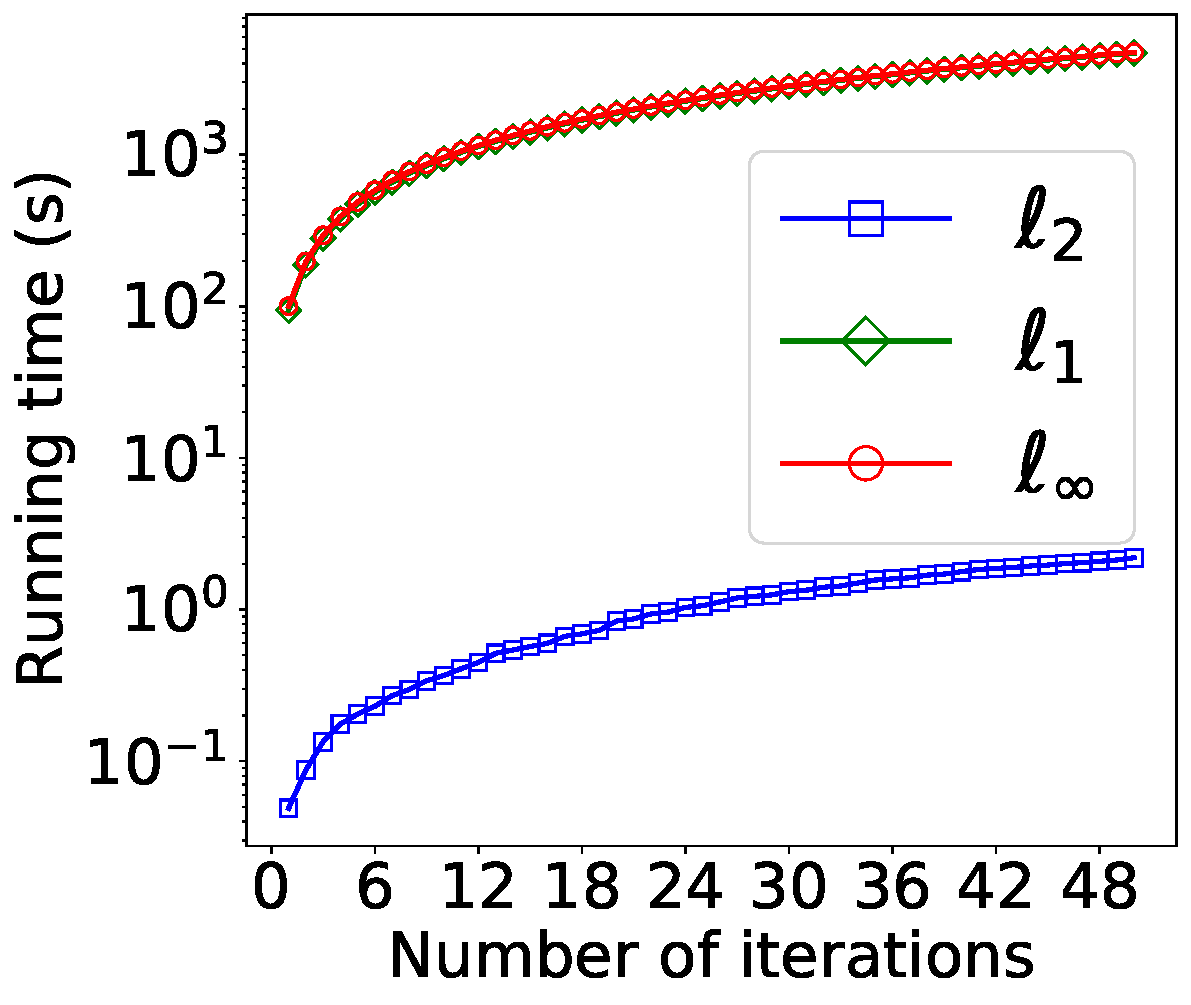
\includegraphics[width=0.33\linewidth]{figures/Linf/time/Linf_Coil.pdf}}
    \subfloat[YALE (sp-10-30-50)] {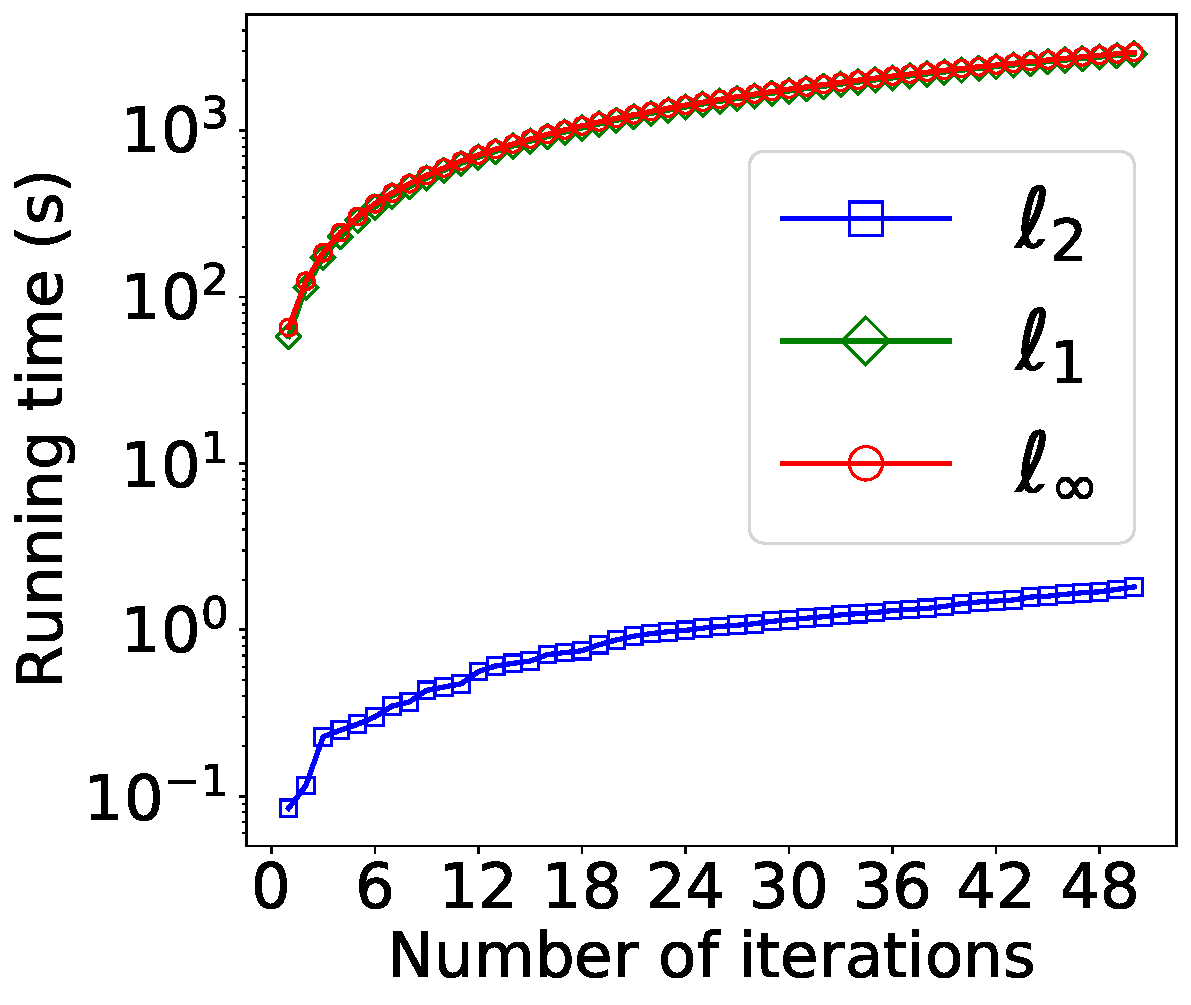
\includegraphics[width=0.33\linewidth]{figures/Linf/time/Linf_Yale.pdf}}
    \subfloat[UMIST (sp-10-30-50)] {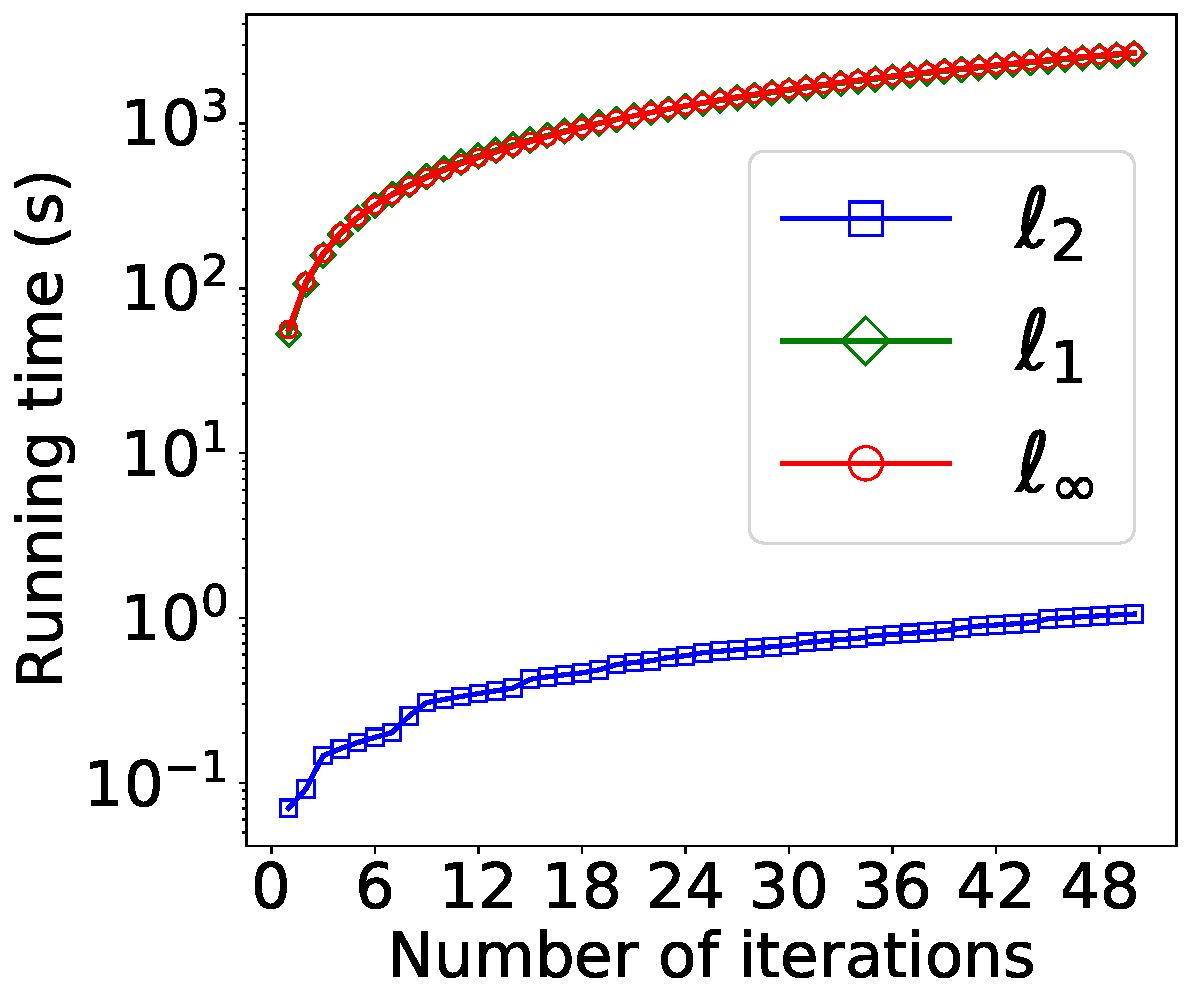
\includegraphics[width=0.33\linewidth]{figures/Linf/time/Linf_Umist.pdf}}
    \caption{Running time analysis on the COIL (sp-10-30-50), YALE (sp-10-30-50) and UMIST (sp-10-30-50) datasets.}
    \label{fig:runt}
\end{figure}
    
\begin{figure}[!ht]
    \centering
    \subfloat[COIL (sp-10-30-50)] {\includegraphics[width=0.33\linewidth]{figures/Linf/loss/loss_coil.pdf}}
    \subfloat[YALE (sp-10-30-50)] {\includegraphics[width=0.33\linewidth]{figures/Linf/loss/loss_yale.pdf}}
    \subfloat[UMIST (sp-10-30-50)] {\includegraphics[width=0.33\linewidth]{figures/Linf/loss/loss_umist.pdf}}
    \caption{Convergence analysis on the COIL (sp-10-30-50), YALE (sp-10-30-50) and UMIST (sp-10-30-50) datasets.}
    \label{fig:conv}
\end{figure}